%  -----------------------------------------------------------------------------
%  Author         : Bimalka Piyaruwan Thalagala
%  GitHub         : https://github.com/bimalka98
%  Date Created   : 01.09.2020
%  Last Modified  : 13.09.2020
%  -----------------------------------------------------------------------------

\documentclass[a4paper,11pt]{article}%,twocolumn
%% packages

\usepackage{blindtext} % needed for creating dummy text passages
%\usepackage{ngerman} % needed for German default language
\usepackage{amsmath} % needed for command eqref
\usepackage{amssymb} % needed for math fonts
\usepackage[colorlinks=true,breaklinks]{hyperref} % needed for creating hyperlinks in the document, the option colorlinks=true gets rid of the awful boxes, breaklinks breaks lonkg links (list of figures), and ngerman sets everything for german as default hyperlinks language
\usepackage[hyphenbreaks]{breakurl} % ben�tigt f�r das Brechen von URLs in Literaturreferenzen, hyphenbreaks auch bei links, die �ber eine Seite gehen (mit hyphenation).
\usepackage{xcolor}
\definecolor{c1}{rgb}{0,0,1} % blue
\definecolor{c2}{rgb}{0,0.3,0.9} % light blue
\definecolor{c3}{rgb}{0.3,0,0.9} % red blue
\hypersetup{
    linkcolor={c1}, % internal links
    citecolor={c2}, % citations
    urlcolor={c3} % external links/urls
}
%\usepackage{cite} % needed for cite
\usepackage[square,authoryear]{natbib} % needed for cite and abbrvnat bibliography style
\usepackage[nottoc]{tocbibind} % needed for displaying bibliography and other in the table of contents
\usepackage{graphicx} % needed for \includegraphics 
\usepackage{longtable} % needed for long tables over pages
\usepackage{bigstrut} % needed for the command \bigstrut
\usepackage{enumerate} % needed for some options in enumerate
%\usepackage{todonotes} % needed for todos
\usepackage{makeidx} % needed for creating an index
\makeindex
\usepackage{gensymb}
\usepackage{url}
\usepackage{psfrag}
\usepackage{multirow}
\usepackage{subfigure}
%% page settings

\usepackage[top=15mm, bottom=15mm,left=20mm,right=20mm]{geometry} % needed for page border settings
\parindent=0mm % for space of first line of new text block
\sloppy % for writing with hyphenless justification (tries to)
\hyphenation{} % use hyphenation of tolerance parametershttp://www.jr-x.de/publikationen/latex/tipps/zeilenumbruch.html
\hyphenpenalty=10000
\exhyphenpenalty=10000
\usepackage{fancyhdr} % needed for head and foot options
%% my macros

%% Text fomats
\newcommand{\tbi}[1]{\textbf{\textit{#1}}}

%% Math fonts
\newcommand{\bbA}{\mathbb{A}}
\newcommand{\bbB}{\mathbb{B}}
\newcommand{\bbC}{\mathbb{C}}
\newcommand{\bbD}{\mathbb{D}}
\newcommand{\bbE}{\mathbb{E}}
\newcommand{\bbF}{\mathbb{F}}
\newcommand{\bbG}{\mathbb{G}}
\newcommand{\bbH}{\mathbb{H}}
\newcommand{\bbI}{\mathbb{I}}
\newcommand{\bbJ}{\mathbb{J}}
\newcommand{\bbK}{\mathbb{K}}
\newcommand{\bbL}{\mathbb{L}}
\newcommand{\bbM}{\mathbb{M}}
\newcommand{\bbN}{\mathbb{N}}
\newcommand{\bbO}{\mathbb{O}}
\newcommand{\bbP}{\mathbb{P}}
\newcommand{\bbQ}{\mathbb{Q}}
\newcommand{\bbR}{\mathbb{R}}
\newcommand{\bbS}{\mathbb{S}}
\newcommand{\bbT}{\mathbb{T}}
\newcommand{\bbU}{\mathbb{U}}
\newcommand{\bbV}{\mathbb{V}}
\newcommand{\bbW}{\mathbb{W}}
\newcommand{\bbX}{\mathbb{X}}
\newcommand{\bbY}{\mathbb{Y}}
\newcommand{\bbZ}{\mathbb{Z}}
\usepackage{float}
\usepackage{circuitikz}


\begin{document}

\begin{titlepage}
\center % Center everything on the page

%-------------------------------------------------------------------------------------
%	HEADING SECTIONS
%------------------------------------------------------------------------------------
\textbf{\large Department of Electronic and Telecommunication Engineering}\\[0.5cm]
\textbf{\Large University of Moratuwa, Sri Lanka}\\[1cm]
\textbf{\large EN 2110 - Electronics - III}\\[2cm]

\includegraphics[width=0.3\textwidth]{figures/uomlogo}\\[2cm]

	
%-------------------------------------------------------------------------------------
%	TITLE SECTION
%------------------------------------------------------------------------------------
\textbf{\Huge Group Project - Group 37}\\[0.5cm]
\textbf{\Large Project Report}\\[5cm]


%----------------------------------------------------------------------------------------
%	MEMBERS SECTION
%----------------------------------------------------------------------------------------

\textbf{\large Submitted by}\\[0.5cm]
\begin{minipage}{0.2\textwidth}
	\begin{flushleft}	   
		{\large Caldera H. D. J.}\\[4mm]
		{\large Oshan J. W. P.}\\[4mm]
		{\large Thalagala B.P.}\\[4mm]
		
	\end{flushleft}
\end{minipage}
\hspace{5mm}
\begin{minipage}{0.2\textwidth}
	\begin{flushright}
		{\large 180079X}\\[4mm]
		{\large 180437U}\\[4mm]
		{\large 180631J }\\[4mm]
		
	\end{flushright}
\end{minipage}\\[1.5cm]

%----------------------------------------------------------------------------------------
%	DATE SECTION
%----------------------------------------------------------------------------------------
\textbf{\large Submitted on}\\[0.5cm]
\textbf{\Large \today} % Date, change the \today to a set date if you want to be precise

%----------------------------------------------------------------------------------------

\vfill % Fill the rest of the page with whitespace

\end{titlepage}
\pagebreak

\begin{table}[H]
		\centering
		\begin{tabular}{l c l}
		\textbf{Name} & \textbf{Index} & \textbf{Contribution}\\

	Caldera H. D. J. &  180079X& \\
	Oshan J. W. P.    & 180437U& \\
	Thalagala B.P. & 180631J & \\


		\end{tabular}
		\caption{Contributions of each member}
\end{table}


\tableofcontents

\pagebreak
\section{Parasitic effect in Timing analysis}
\textbf{Objective}: \textit{Design a 3 stage (3 inverters) ring oscillator. Find the correlation of the parasitic effect in the oscillation period.}\\

\subsection{System Design}
Ring oscillator is a combination of delay stages arranged in series to form a closed loop chain. It consists of an \textbf{\textit{odd number of identical inverters (NOT gates)}} and it has an periodically oscillating output. The period of oscillation($T$) of a ring oscillator can be expressed as follows where $n$ is the number of cascaded NOT gates and $\tau_{d}$ is the propagation delay of a single inverter(per stage).

\[
T = 2.n.\tau_{d} \hspace{5mm}\Longrightarrow ~ Oscillation~frequency = \frac{1}{2.n.\tau_{d}}
\]

Following figure illustrates the input output characteristic of an ideal inverter. There, output is changed as soon as the input signal changes.

\begin{figure}[H]
	\centering
	\subfigure[Ideal Inverter Model]
	{ 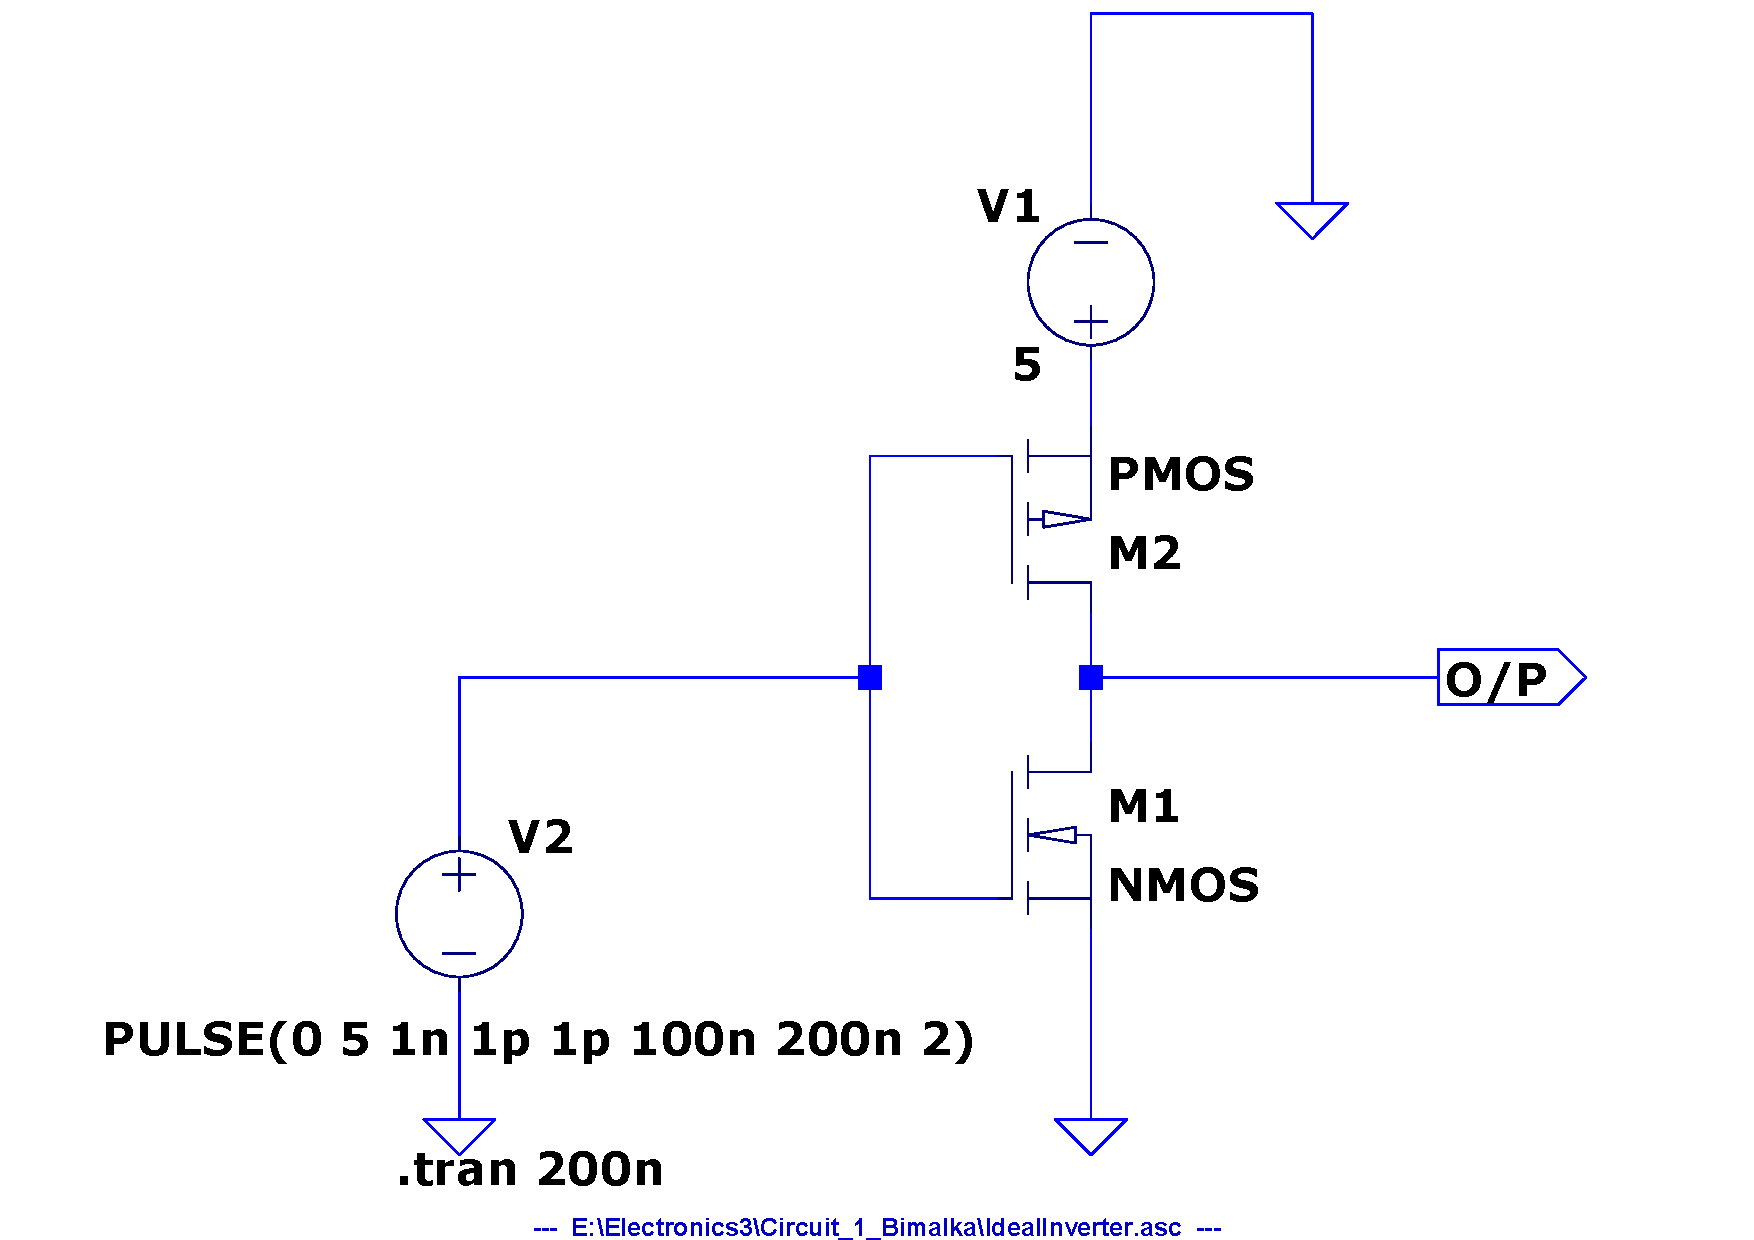
\includegraphics[scale=0.25]{figures/cct1plot5}
	}\hfill
	\subfigure[Ideal inverter Output]
	{ 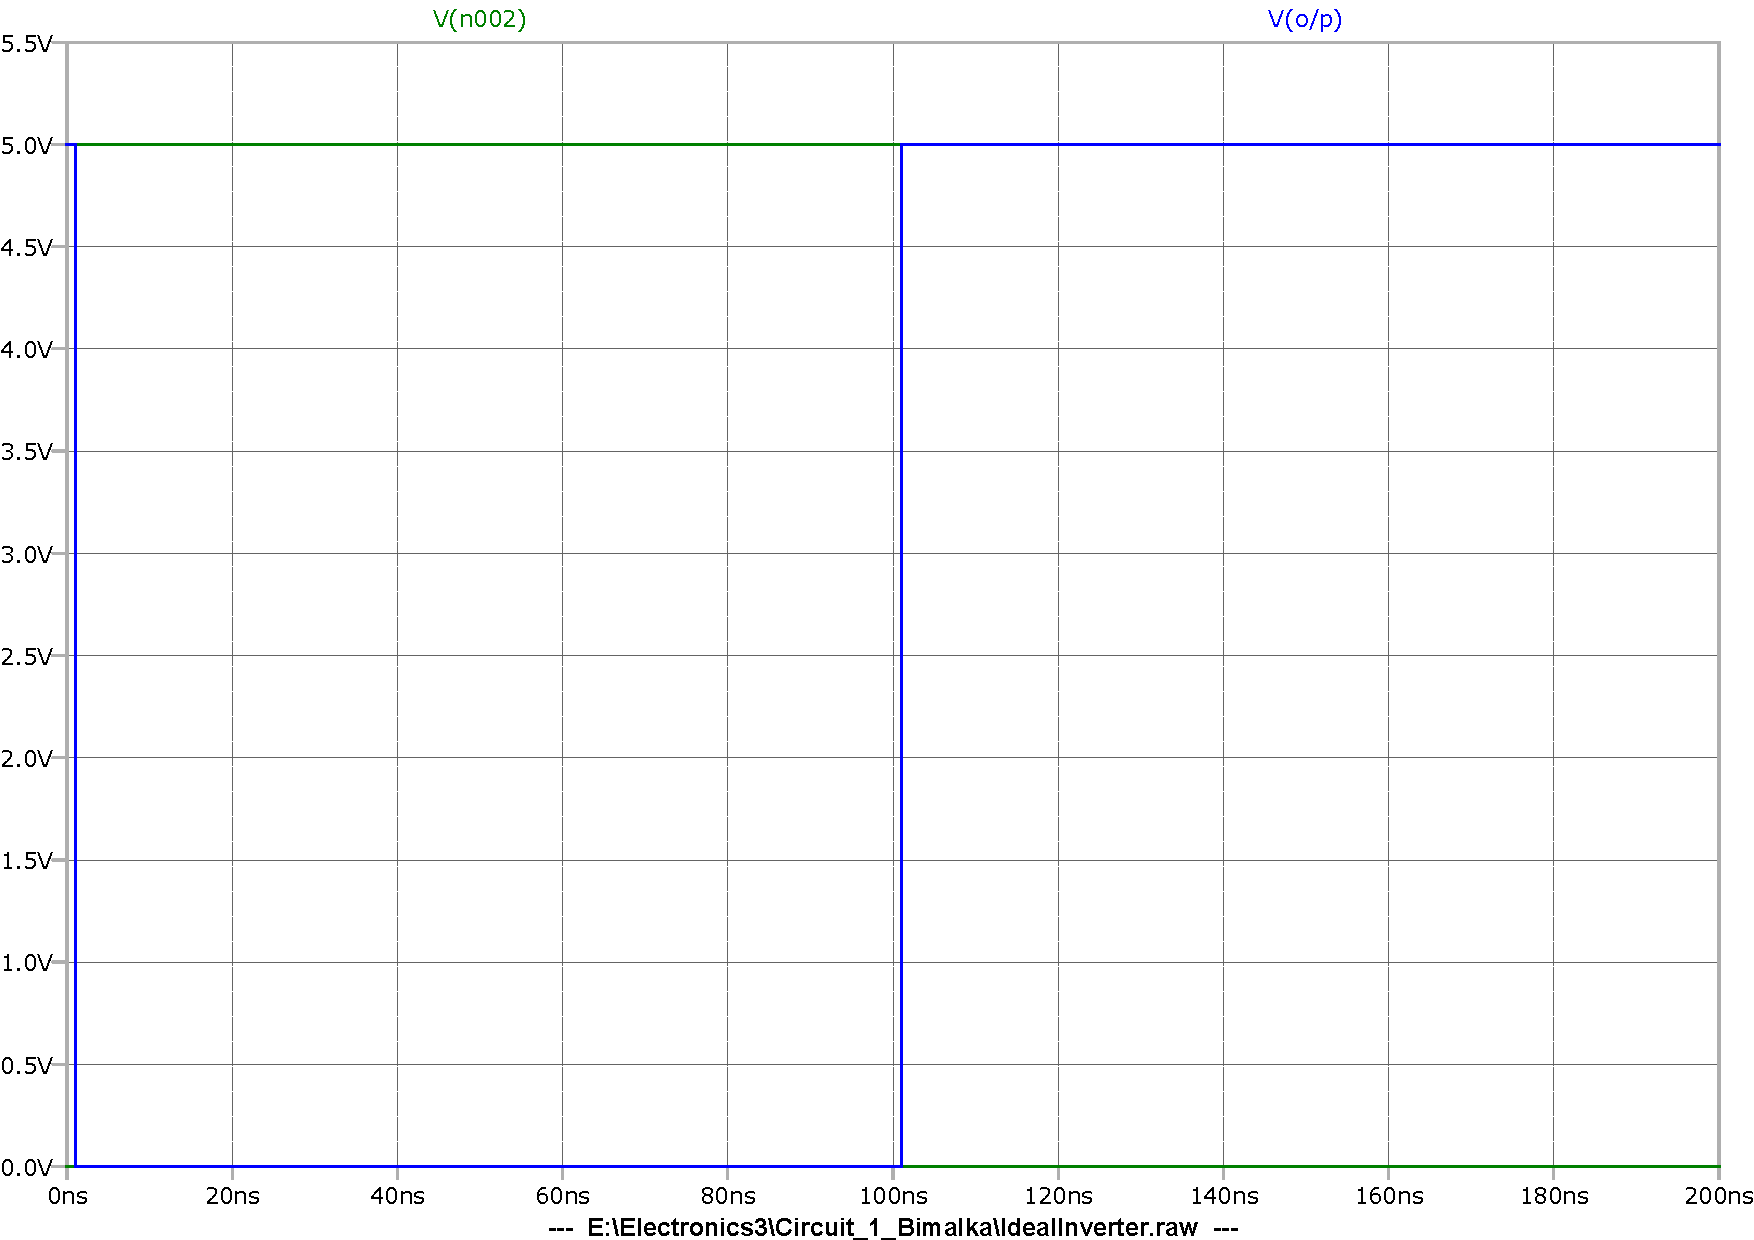
\includegraphics[scale=0.25]{figures/cct1plot6}
	}
\end{figure}

Whereas the below figure illustrates the input output characteristic of a single stage of a general Ring Oscillator. It can be observed that finite amount of time delay is required for output to be valid for a given valid input.

\begin{figure}[H]
	\subfigure[Inverter Model with additional delay element]
	{ 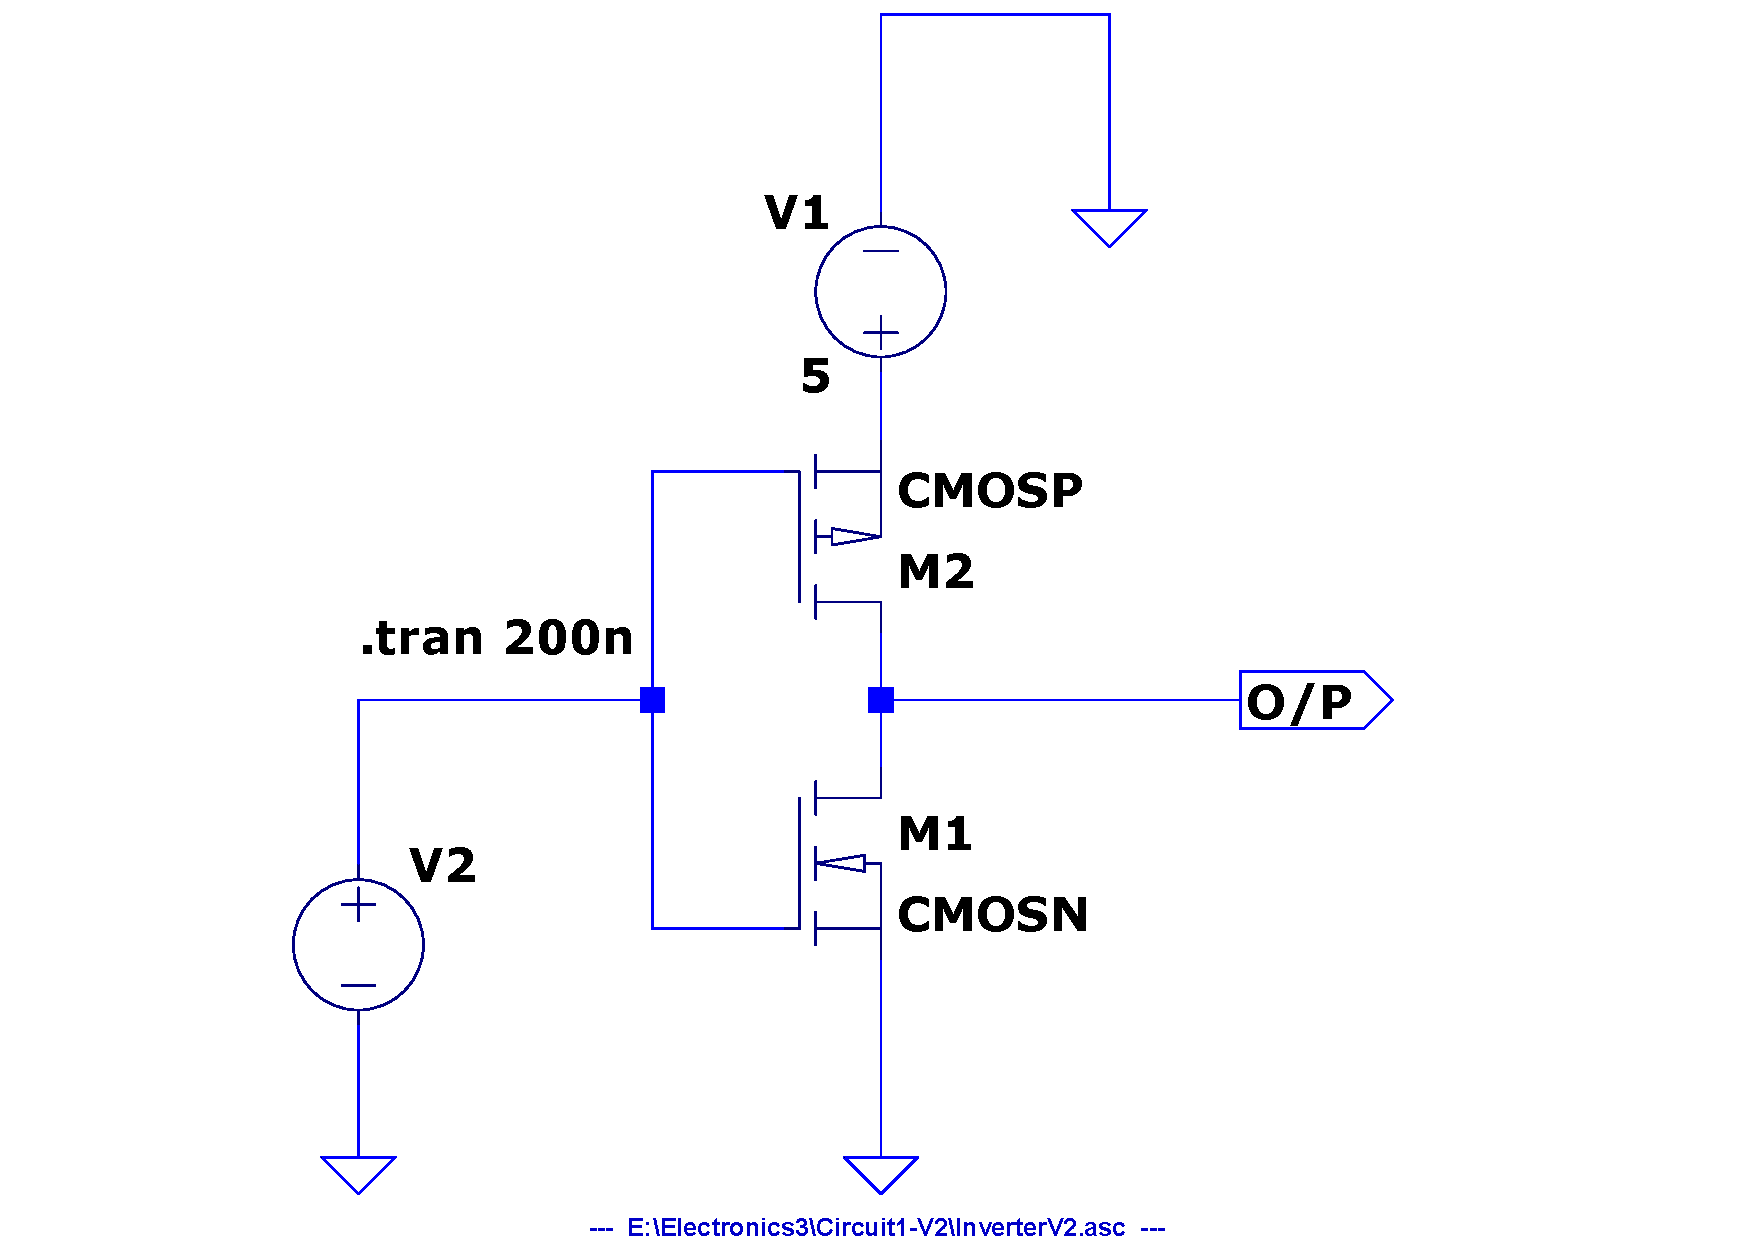
\includegraphics[scale=0.25]{figures/cct1plot3}
	}\hfill
	\subfigure[Effect of Parasitic Capacitance]
	{ 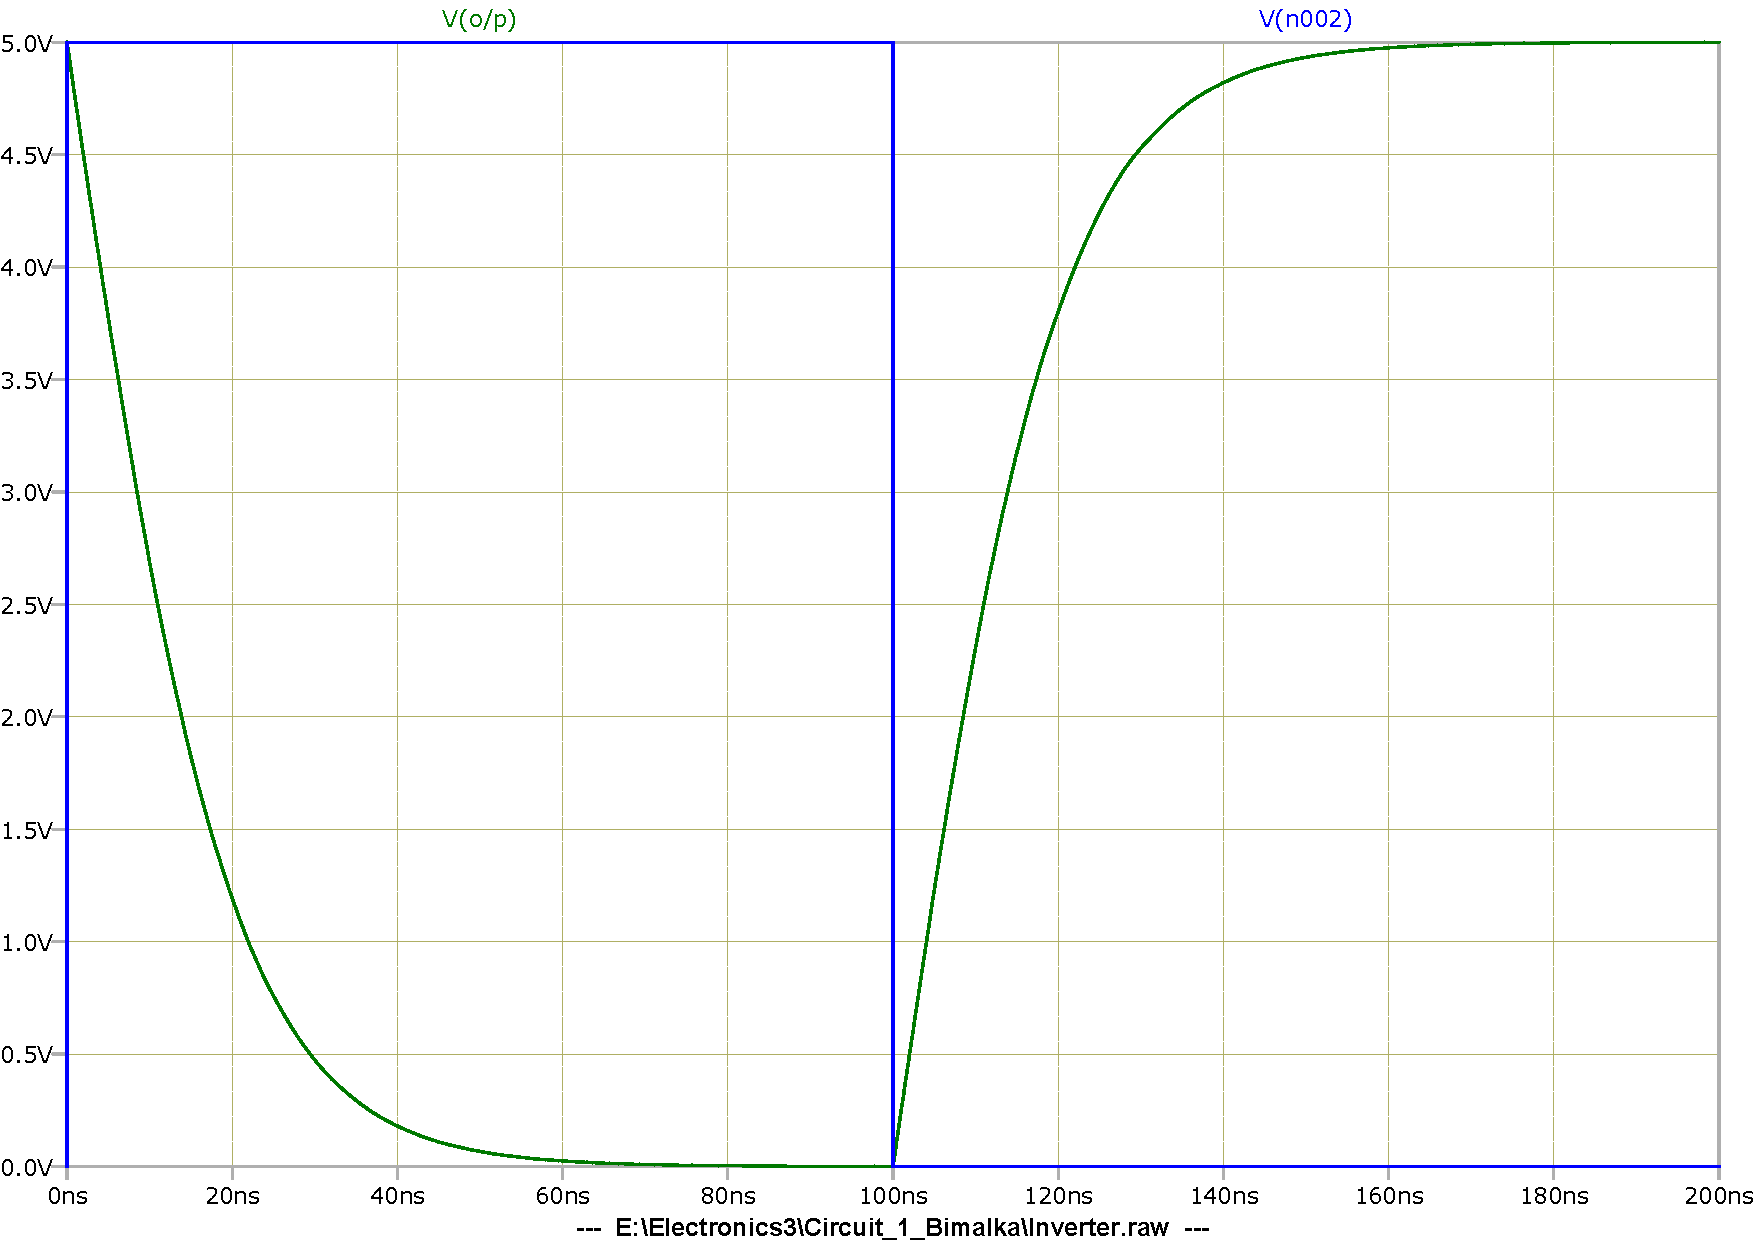
\includegraphics[scale=0.25]{figures/cct1plot4}
	}
\end{figure}

Basic structure of a ring oscillator can be depicted as follows.

\begin{figure}[H]
	\centering
	\begin{circuitikz}
 \draw	 (1,0) node[ieeestd not port] (not1) {}
		 (3,0) node[ieeestd not port] (not2) {}
		 (5,0) node[ieeestd not port] (not3) {}
		 (0,0) -- (not1.in)
		 (not2.in) -- (not1.out)
		 (not3.in) -- (not2.out)
		 (not3.out) -- (6,0)
		 (not1.in) -- (0,0)
		 (6,0) -- (6,-1.5) -- (0,-1.5) -- (0,0) 
		 ;
	\end{circuitikz}
	\caption{Basic structure of a 3 stage ring oscillator}
\end{figure}



This can be implemented using enhanced NMOS and PMOS as illustrated in the following schematic. Each inverter consists of   




\subsection{simulation Results and Discussion}

Following ring oscillator schematic, which was taken from\cite{enwiki:1009565738}  is used to simulate the effect of parasitic capacitance of the CMOS on the period of the output waveform.

\begin{figure}[H]
	\centering
	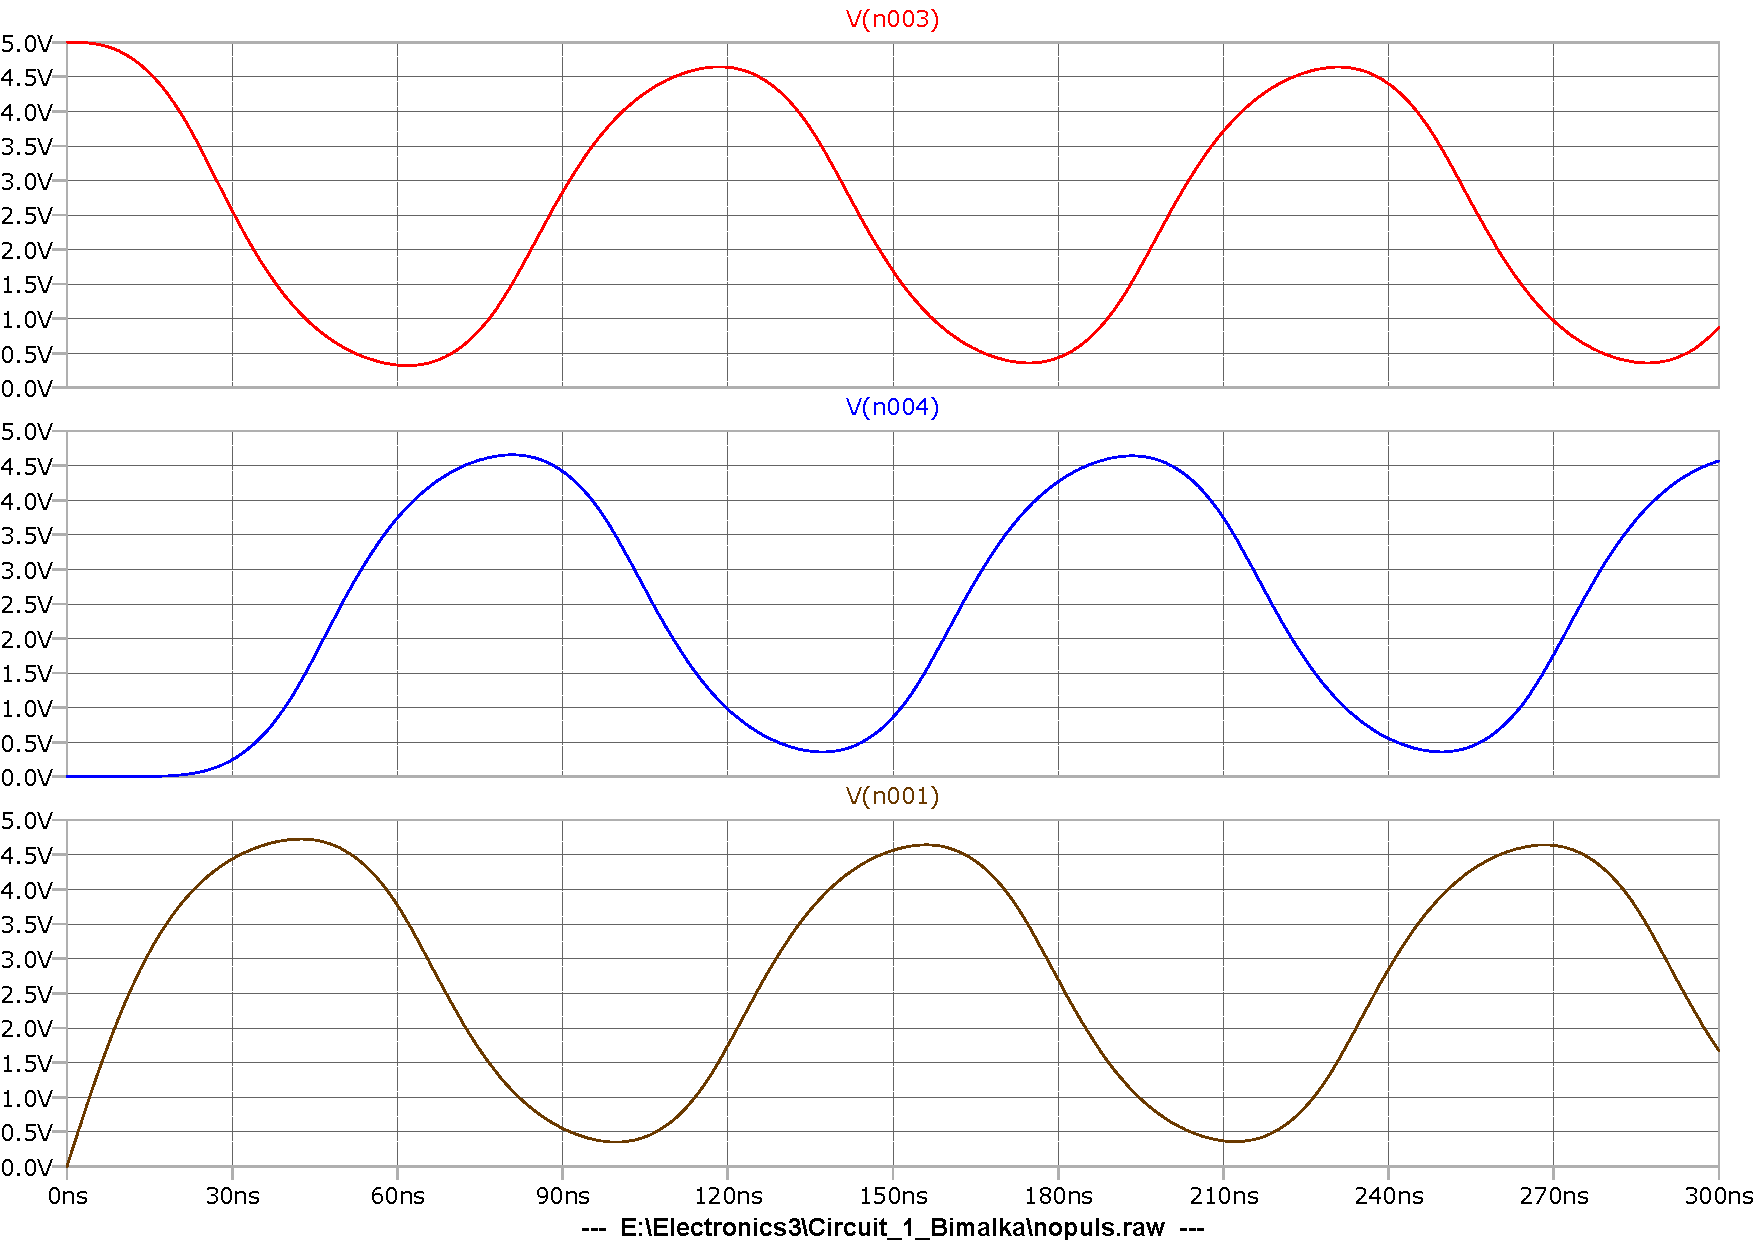
\includegraphics[scale=0.5]{figures/cct1plot1}
	\caption{3 stages enhanced CMOS Ring Oscillator}
\end{figure}

\begin{figure}[H]
	\centering
	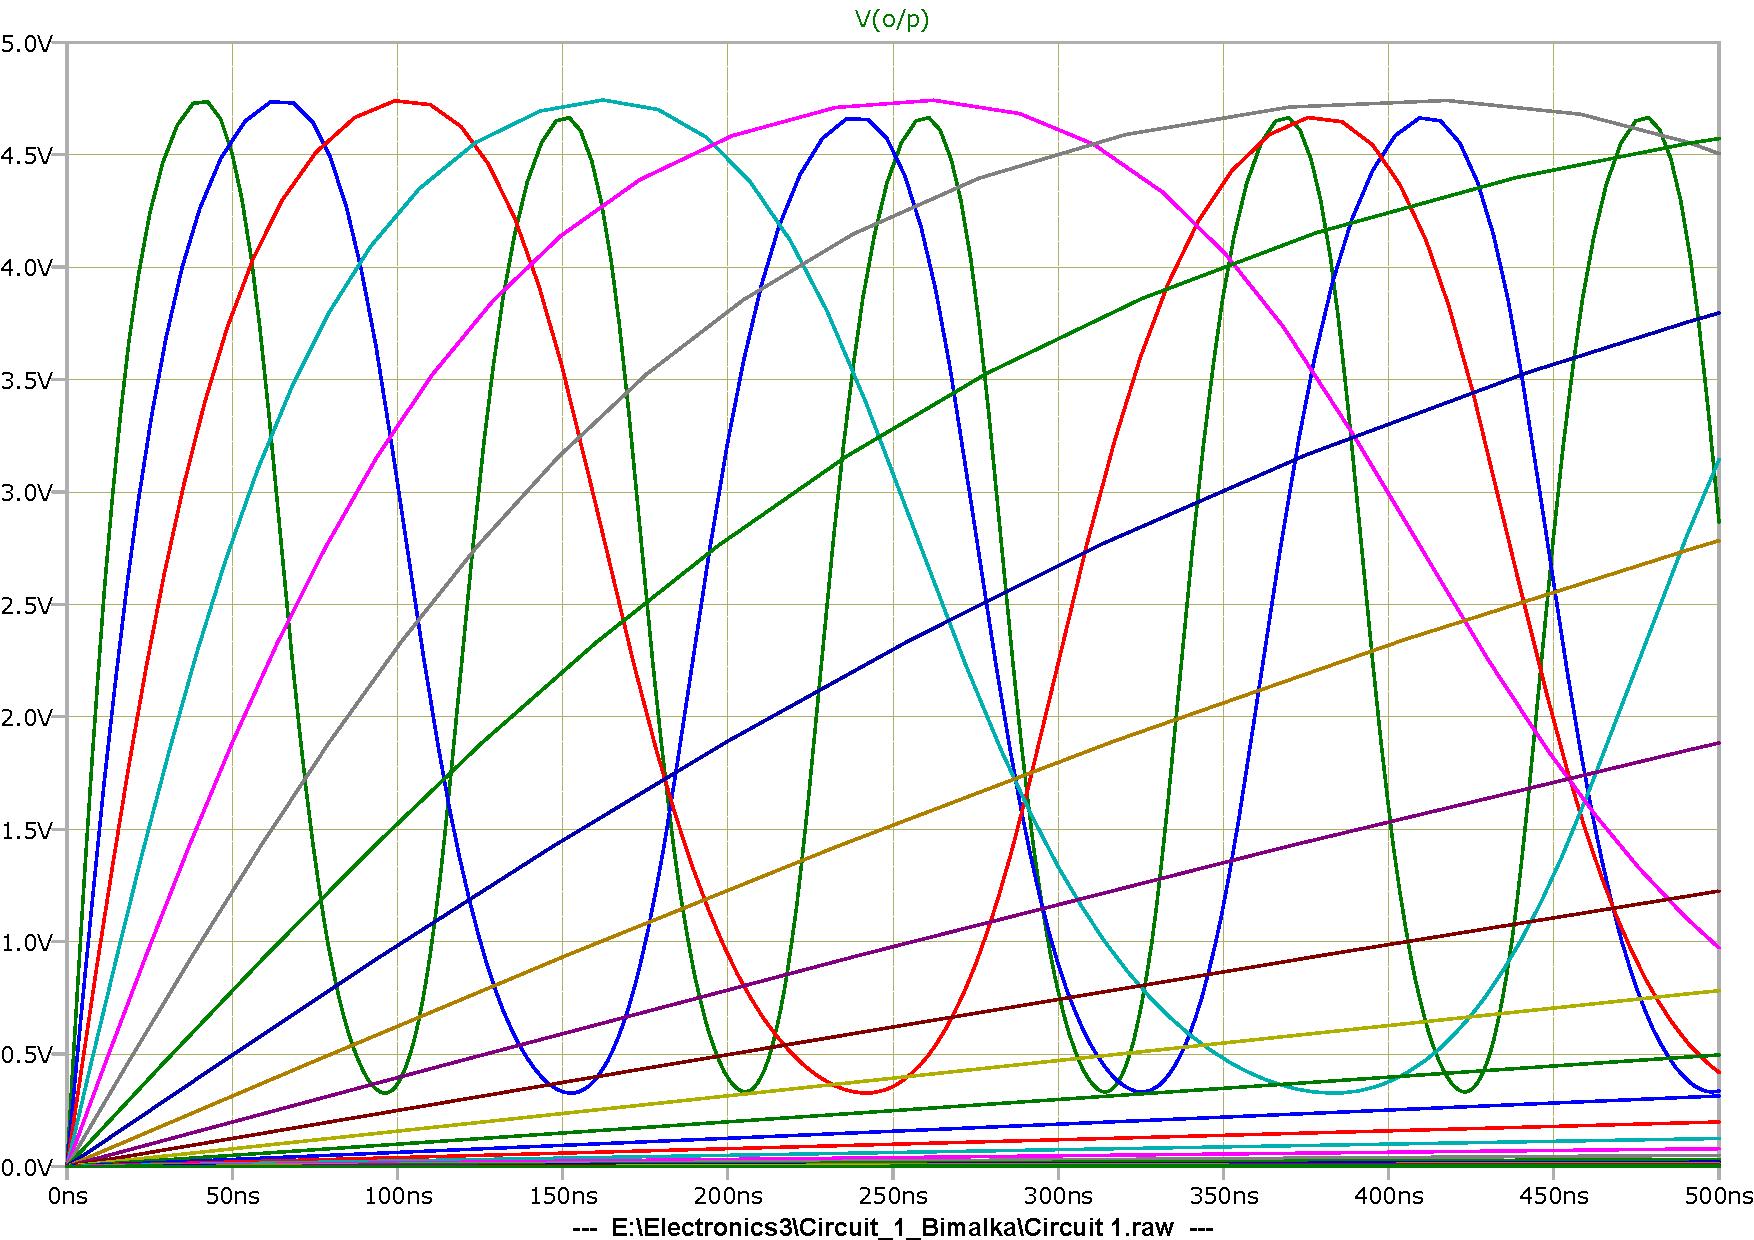
\includegraphics[scale=0.5]{figures/cct1plot2}
	\caption{Waveform for Voltages of 3 stages enhanced CMOS Ring Oscillator}
\end{figure}


\pagebreak
\section{PLD}
\subsection{Part 1}
\textbf{Objective}: \textit{Design a programmable logic block to configure it as a `NAND' or a `NOR' gate using a single selection bit.}\\

First a truth table is drawn for this part considering a single selection bit (S) with two inputs (A, B) such that S=0 for ‘NAND’ and S=1 for ‘NOR’ operations respectively.
\begin{table}[H]
	\centering
	\begin{tabular}{|c |c| c| c|}
		\hline
		S & A & B & F \\\hline
		0 & 0 & 0 & 1 \\
		0 & 0 & 1 & 1 \\
		0 & 1 & 0 & 1 \\
		0 & 1 & 1 & 0 \\\hline
		1 & 0 & 0 & 1 \\
		1 & 0 & 1 & 0 \\
		1 & 1 & 0 & 0 \\
		1 & 1 & 1 & 0 \\\hline\hline
	\end{tabular}
\caption{The truth table}
\end{table}

Then the relevant logic expression was obtained using a karnaugh map and it was further simplified to obtain the combination of 'NAND' and 'NOR' operations.

\begin{table}[H]
	\centering
	\begin{tabular}{c |c| c| c| c}
		S\textbackslash AB & 00 & 01 & 11 & 10\\\hline
		0 & 1 & 1 & 0 & 1\\\hline
		1 & 1 & 0  &0  & 0
	\end{tabular}
	\caption{Karnough Map for the above truth table}
\end{table}

\[
\begin{split}
	F &= \overline{S}.\overline{A} + \overline{S}.\overline{B} + \overline{A}.\overline{B}\\
	&= \overline{S}.(\overline{A}+\overline{B}) + \overline{A}.\overline{B}\\
	&= \overline{S}.(\overline{A.B}) + \overline{A+B}\\
	&= \overline{S+A.B} + \overline{A+B}\\
	& = \overline{(S + A.B).(A+B)}\\
	& =\overline{(S + \overline{\overline{A.B}}).(\overline{\overline{A+B}})}
\end{split}
\]



So, the resultant combinational logic circuit is as follows. (2 NANDs, 2 NORs, 3 NOTs) For the implementation of this circuit; ‘NOT’, ‘NAND’, and 'NOR' gates were designed using 'NMOS' and 'PMOS' transistors. Their schematics in LTspice are depicted below.

\begin{figure}[H]
	\centering
	\subfigure[Schematic of NOT gate]
	{ 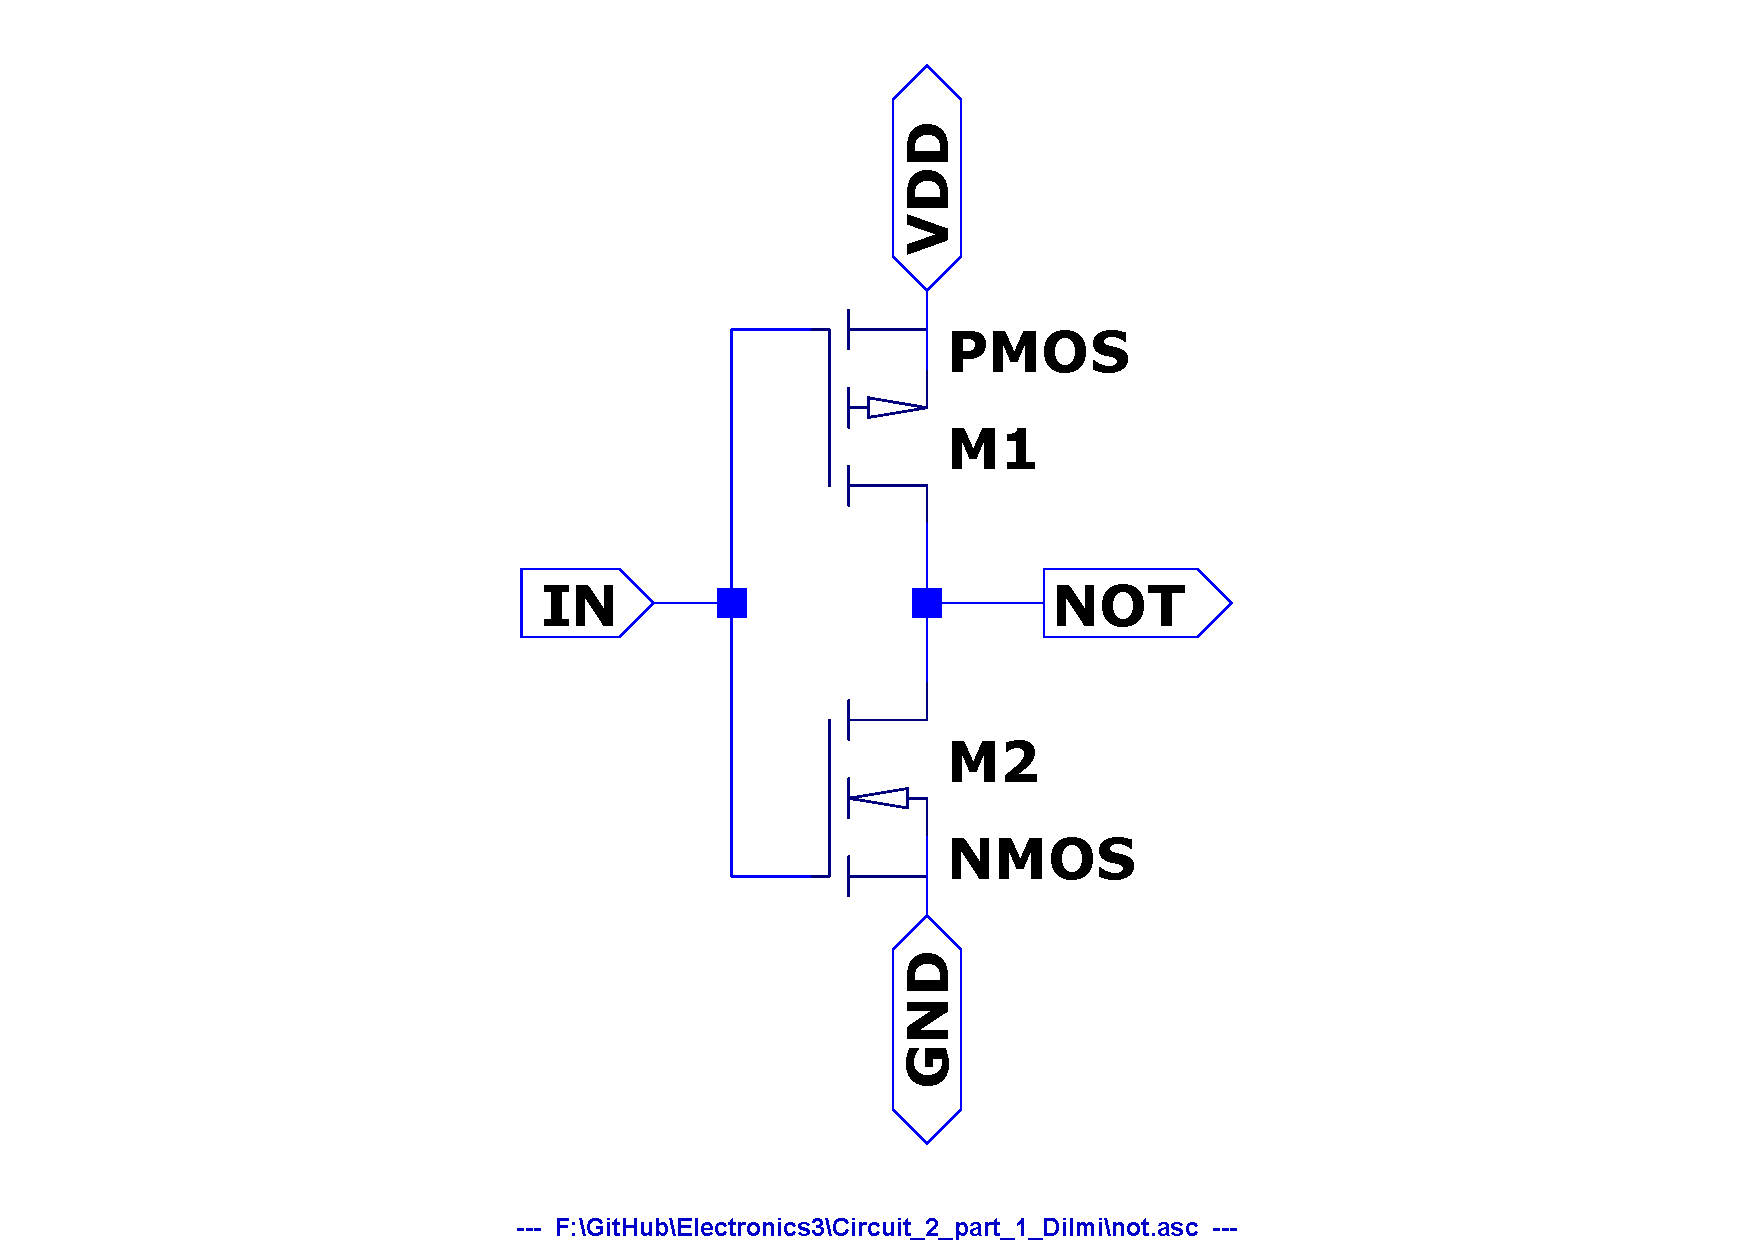
\includegraphics[scale=0.18]{figures/2part1/NOT.pdf}
	}\hfill
	\subfigure[Schematic of NAND gate]
	{ 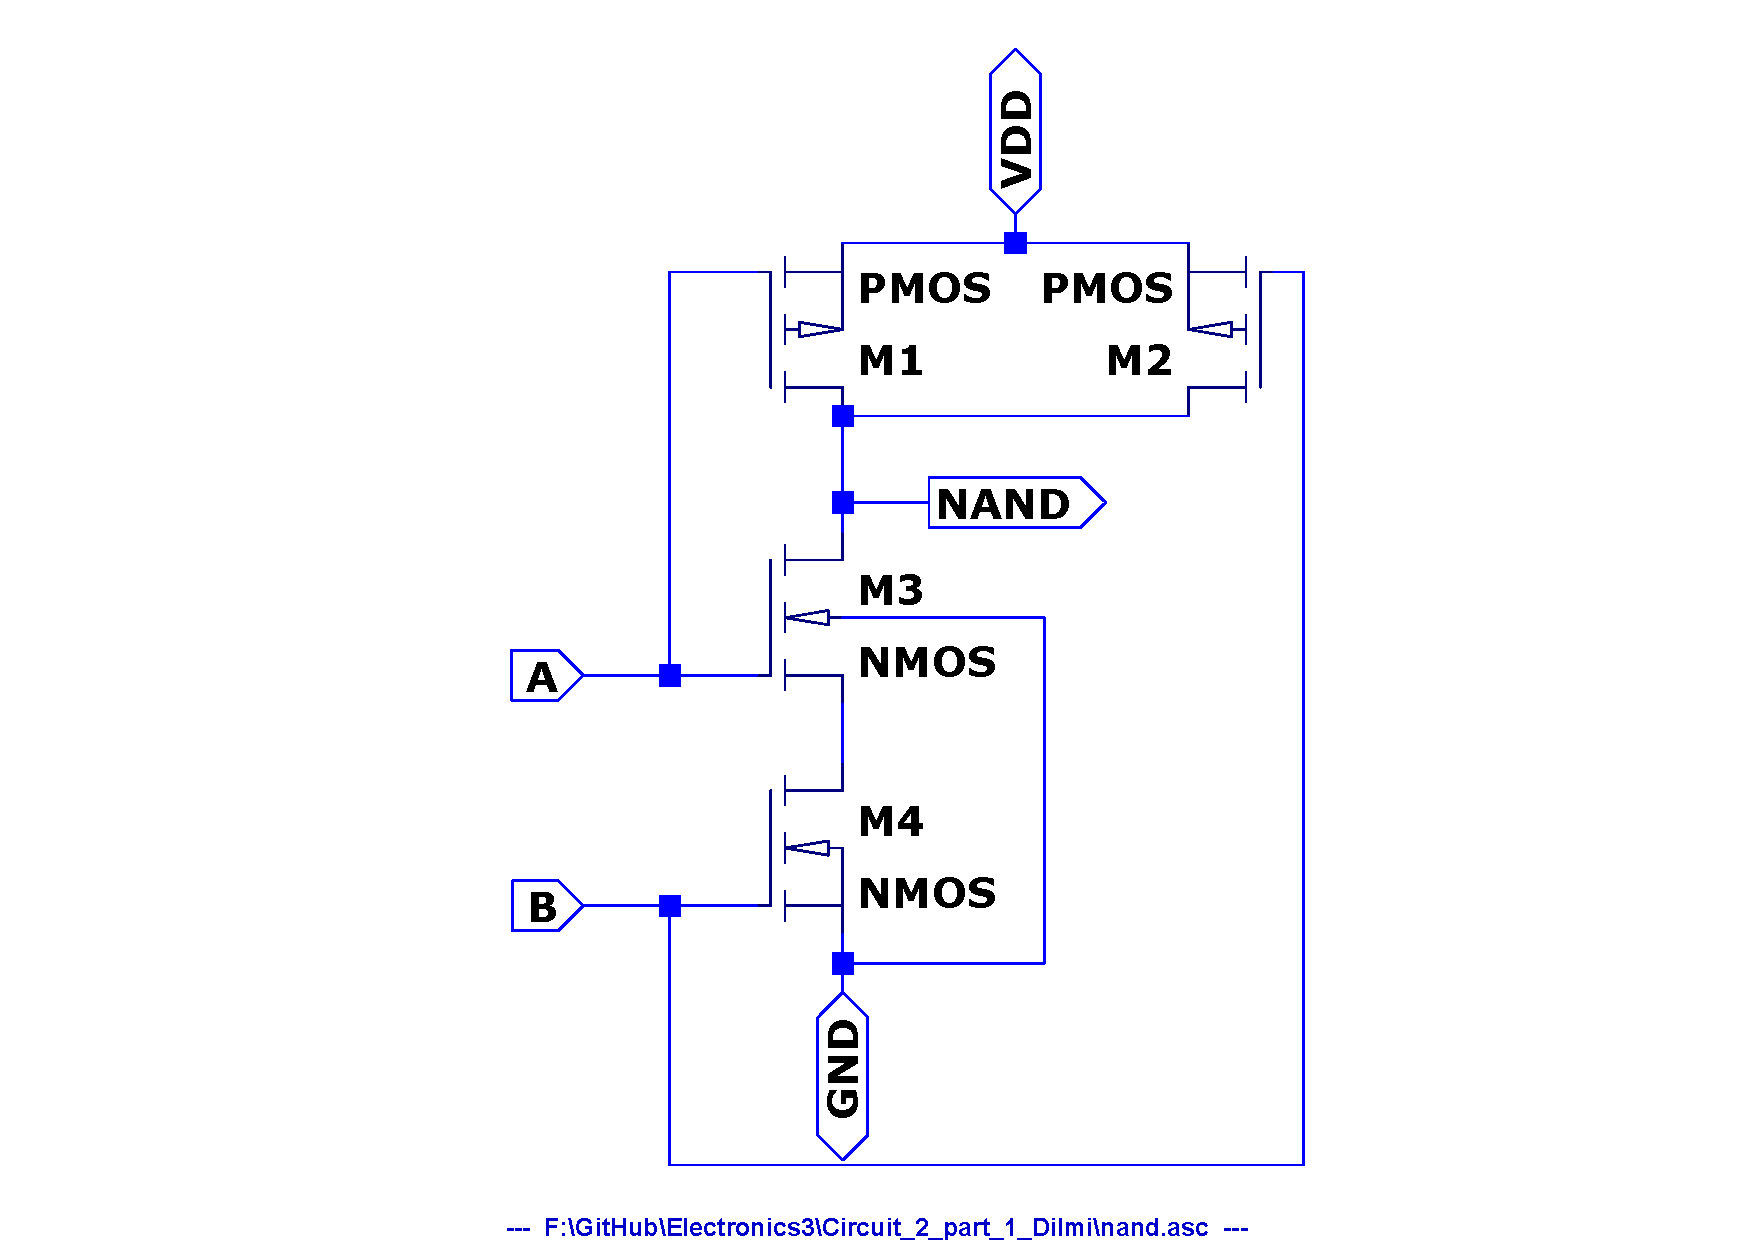
\includegraphics[scale=0.18]{figures/2part1/NAND.pdf}
	}\hfill
	\subfigure[Schematic of NOR gate]
	{ 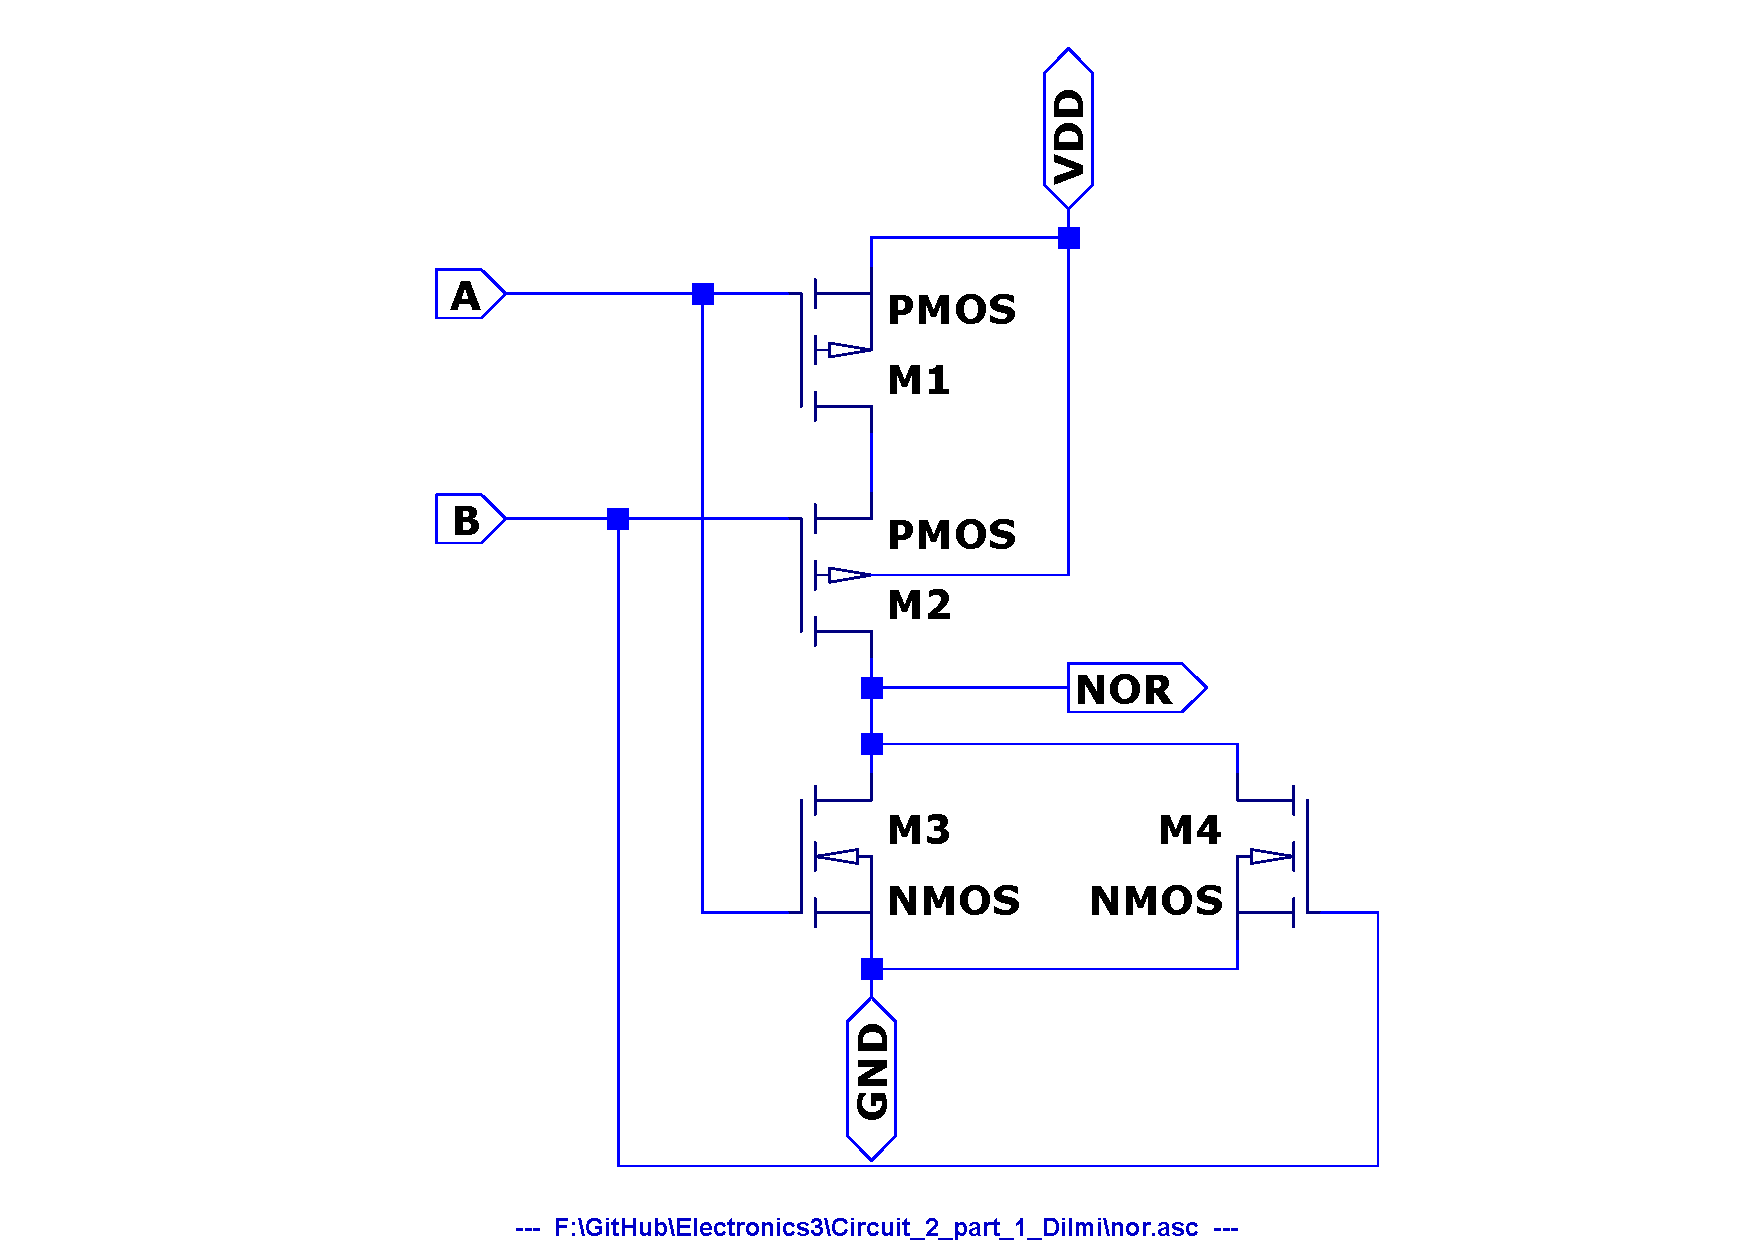
\includegraphics[scale=0.18]{figures/2part1/NOR.pdf}
	}
\caption{Basic Gates in the CMOS logic}
\end{figure}
%
%
Finally, the PLD block is designed using the above gates and the waveforms were obtained.

\begin{figure}[H]
	\centering
	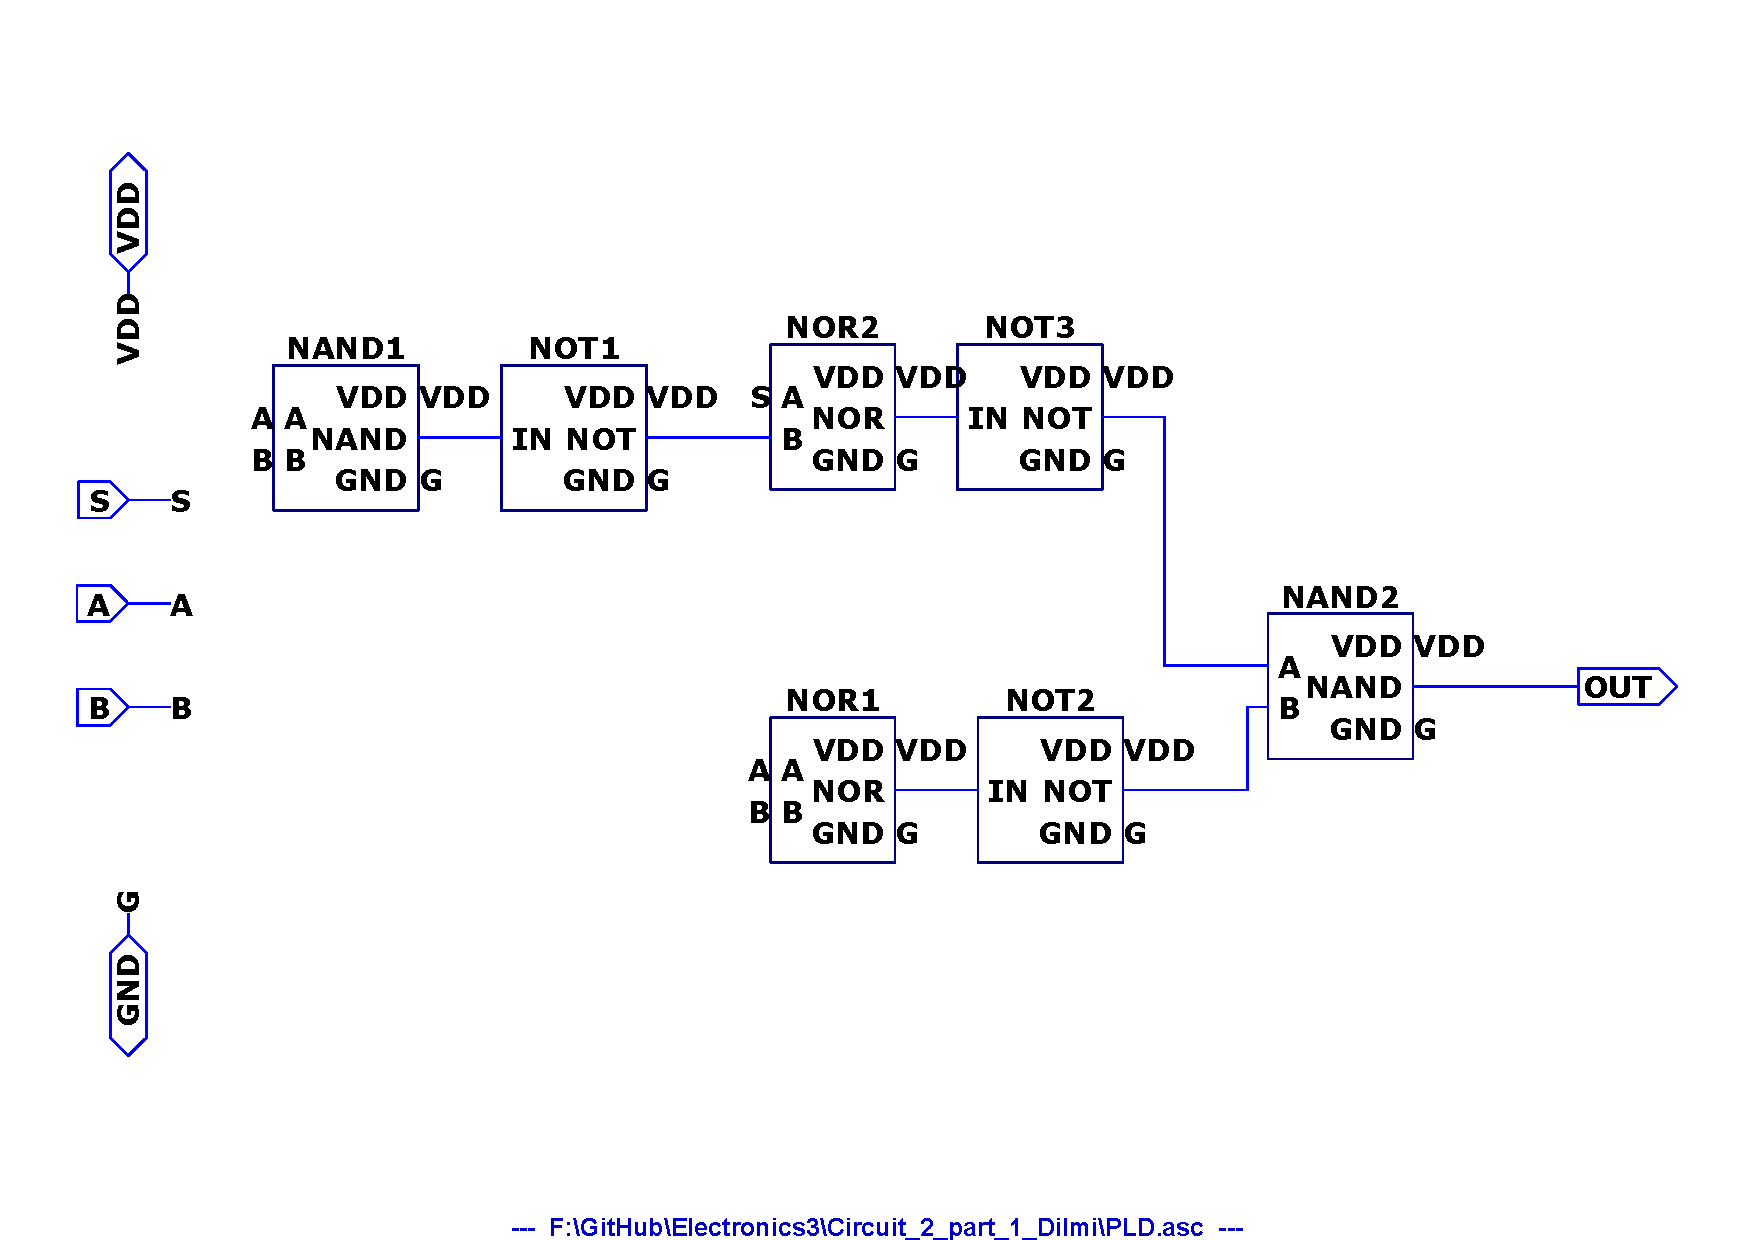
\includegraphics[scale=0.5]{figures/2part1/cct.pdf}
	\caption{Circuit designed using logic blocks}
\end{figure}

\begin{figure}[H]
	\centering
	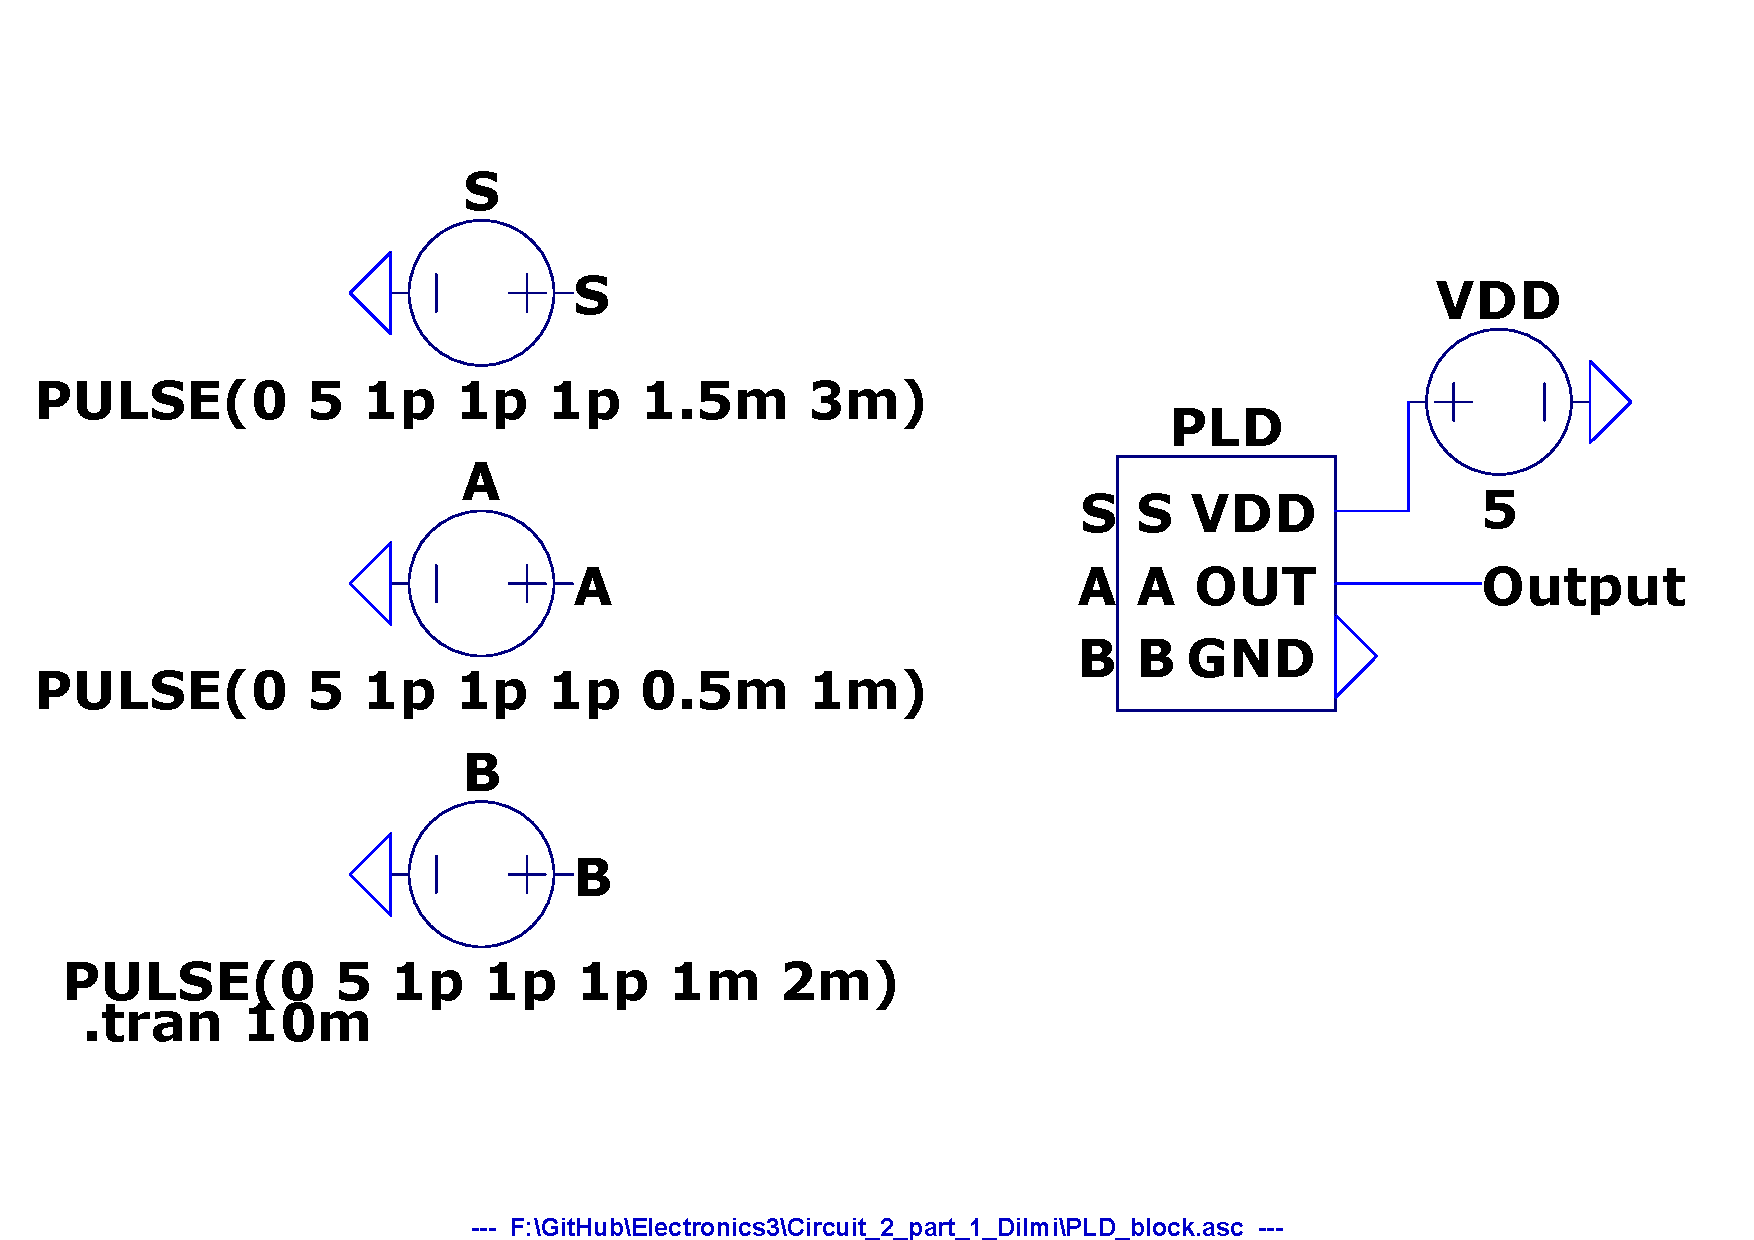
\includegraphics[scale=0.5]{figures/2part1/block.pdf}
	\caption{Designed PLD block}
\end{figure}


\begin{figure}[H]
	\centering
	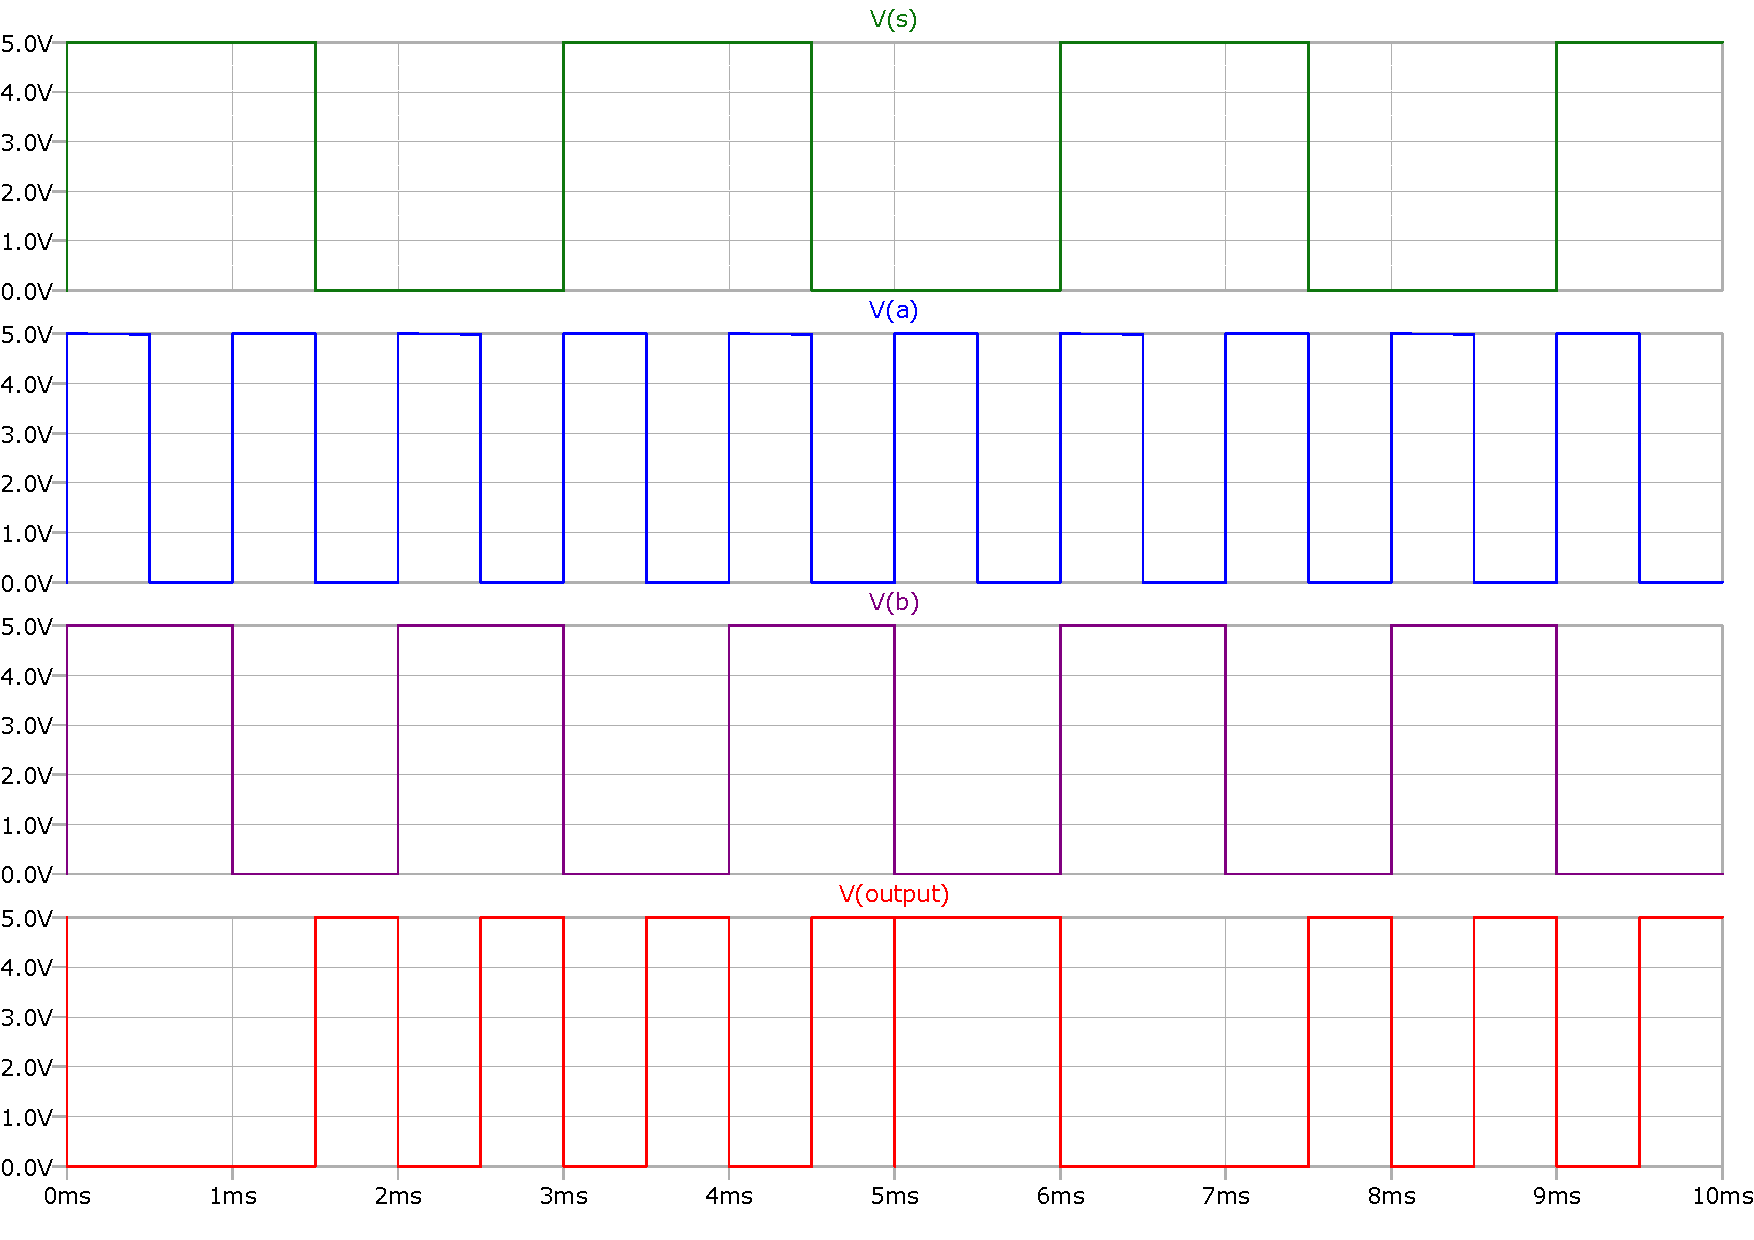
\includegraphics[scale=0.5]{figures/2part1/wave.pdf}
	\caption{Waveforms for inputs and output of PLD }
\end{figure}

\hrule
\subsection{Part 2}
\textbf{Objective}: \textit{Design a single switch matrix using six pass transistors.}\\

In this part, the single switch matrix is needed to be designed using six pass transistors. So as the first step, a pass transistor was designed and its performance was checked. Simply an 'NMOS' transistor is fed with a switch, could be used for this task. So when the switch is on, the input signal will be received at the output (Threshold voltage is considering as zero since an ideal nmos). Also capacitors were used to ground the high impedance state which occurred when the NMOS is OFF.

\begin{figure}[H]
	\centering
	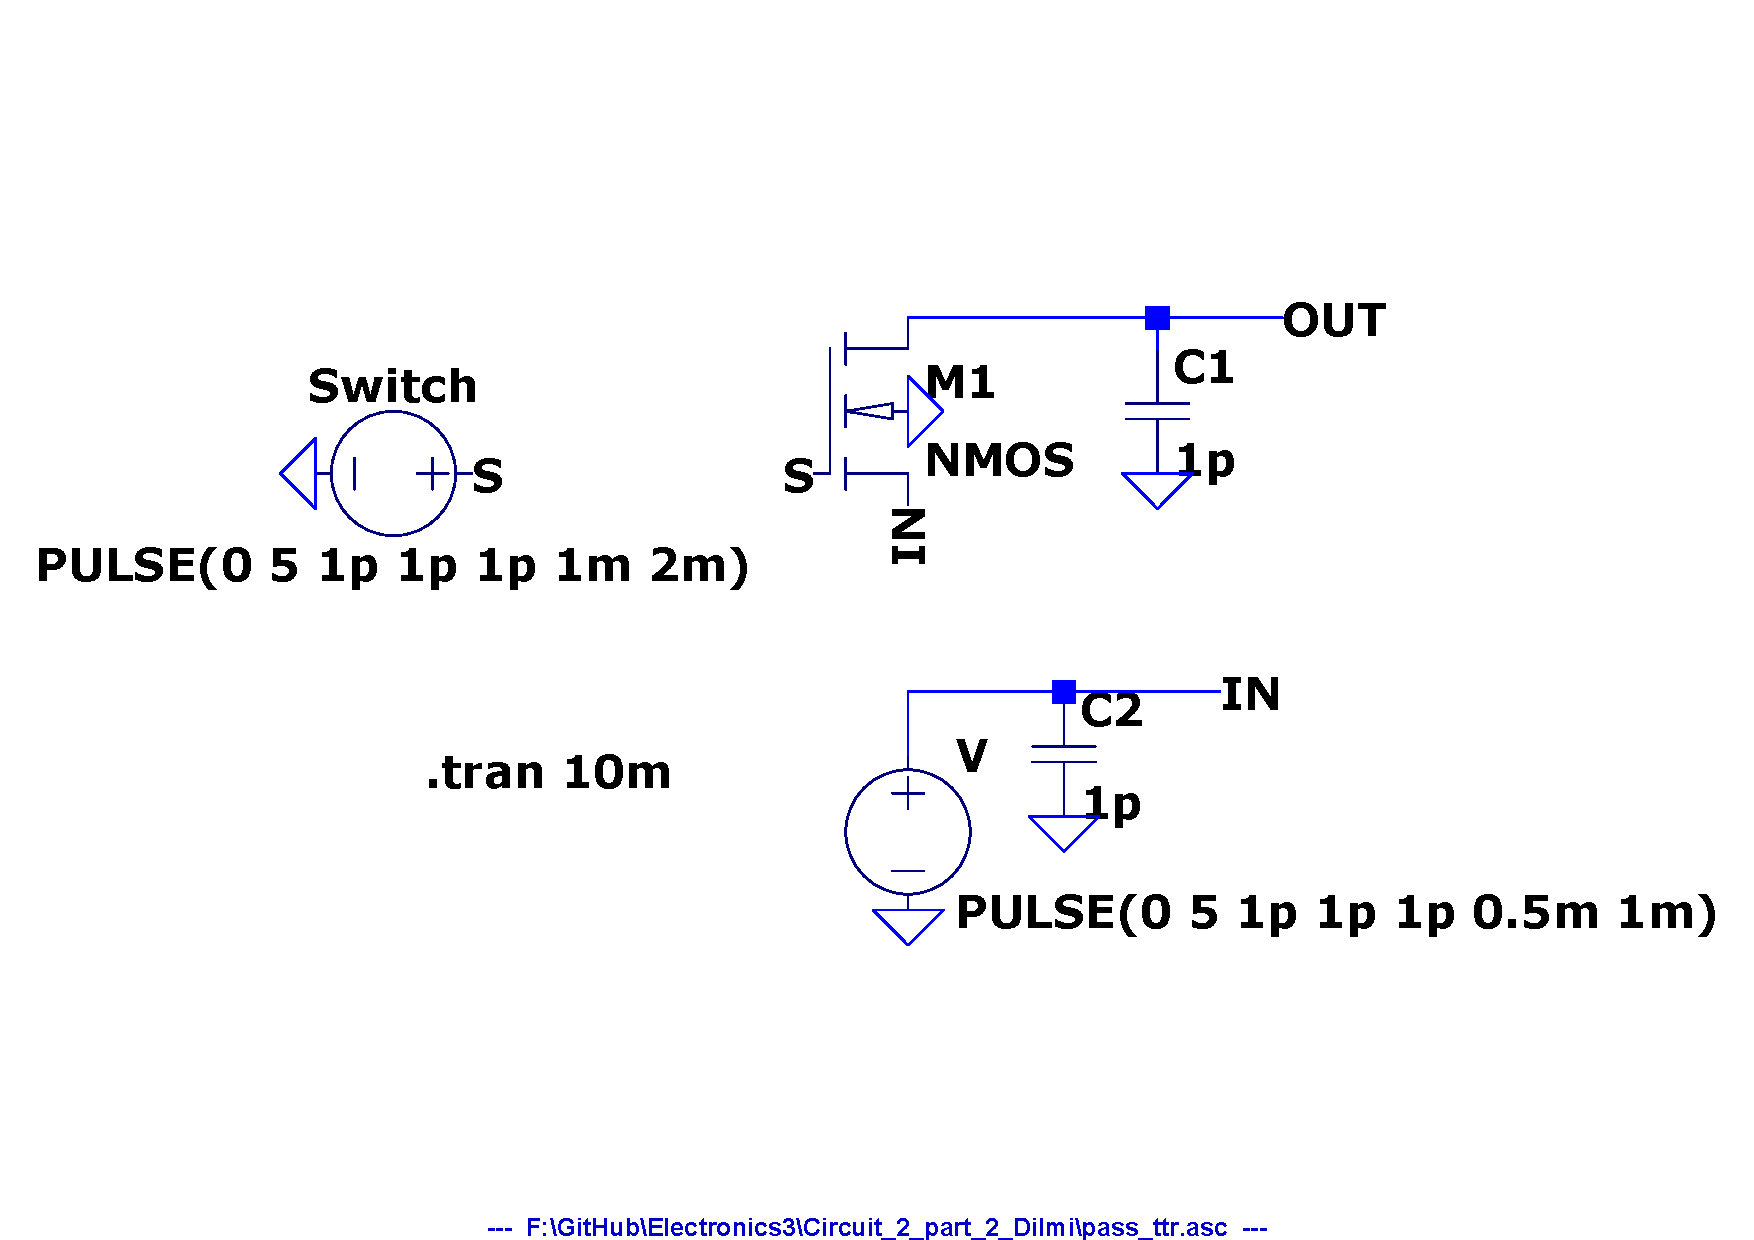
\includegraphics[scale=0.4]{figures/2part2/pass_ttr.pdf}
	\caption{Schematic diagram of the pass transistor}
\end{figure}
\begin{figure}[H]
	\centering
	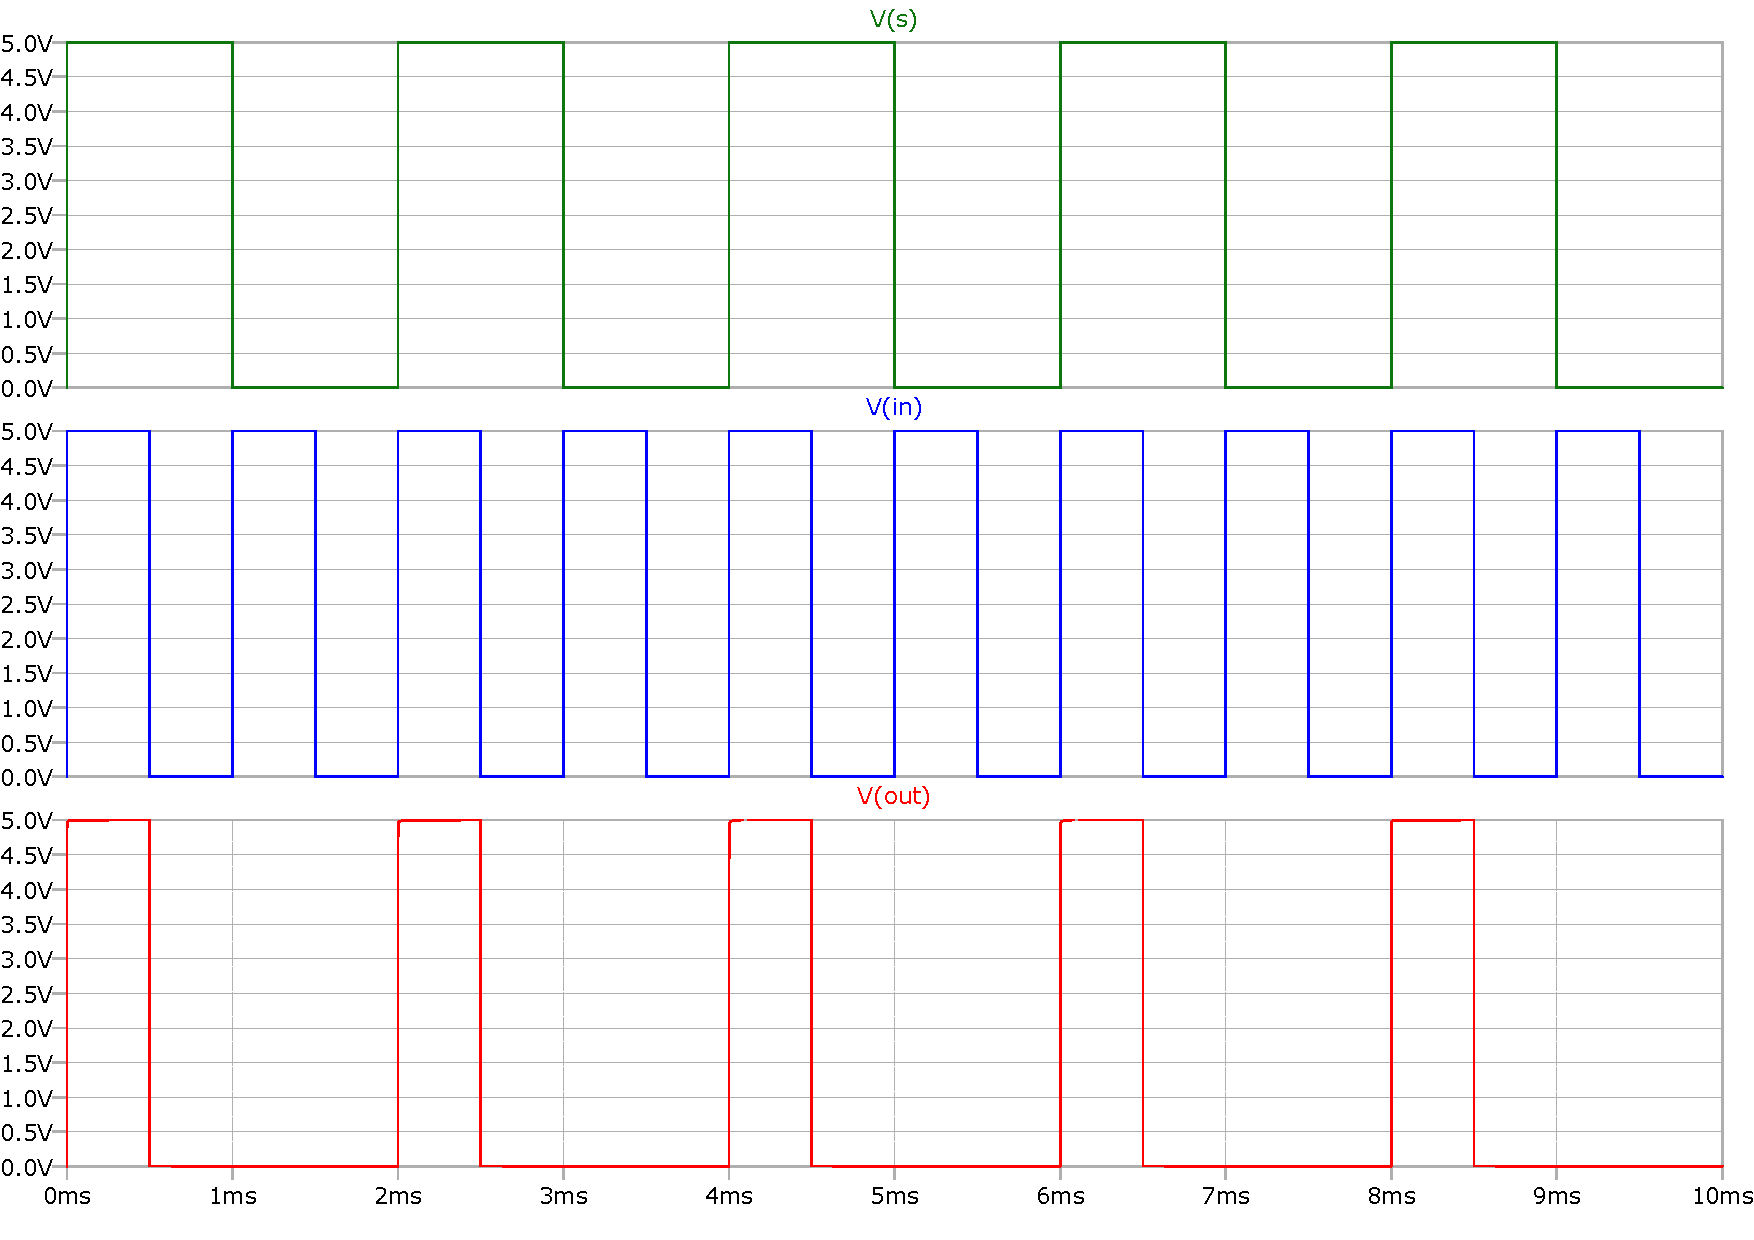
\includegraphics[scale=0.5]{figures/2part2/pass_wave.pdf}
	\caption{Waveform of the pass transistor}
\end{figure}

Then using six such transistors, the single switch matrix was designed and the schematic diagram of it is shown below.

\begin{figure}[H]
	\centering
	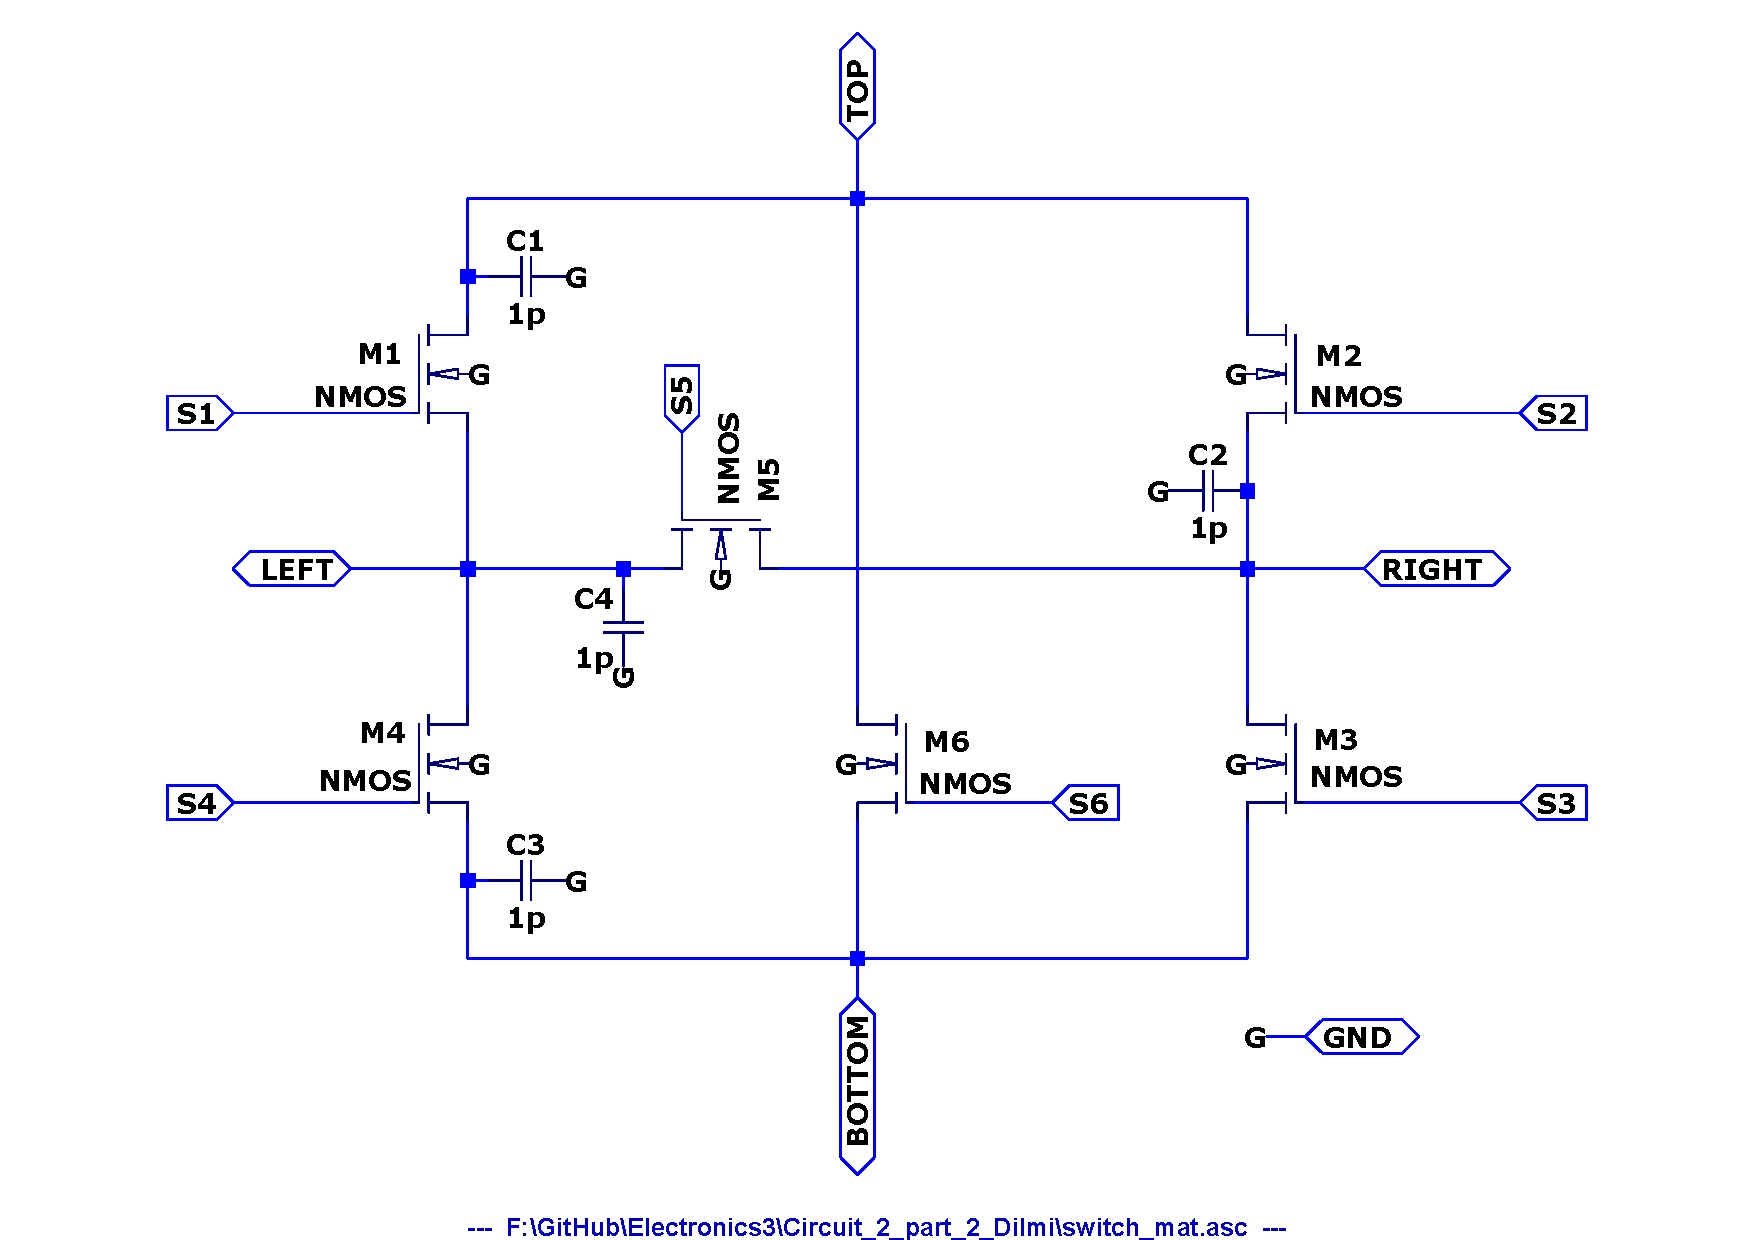
\includegraphics[scale=0.5]{figures/2part2/switch_mat.pdf}
	\caption{Schematic diagram of the single switch matrix}
\end{figure}
\begin{figure}[H]
	\centering
	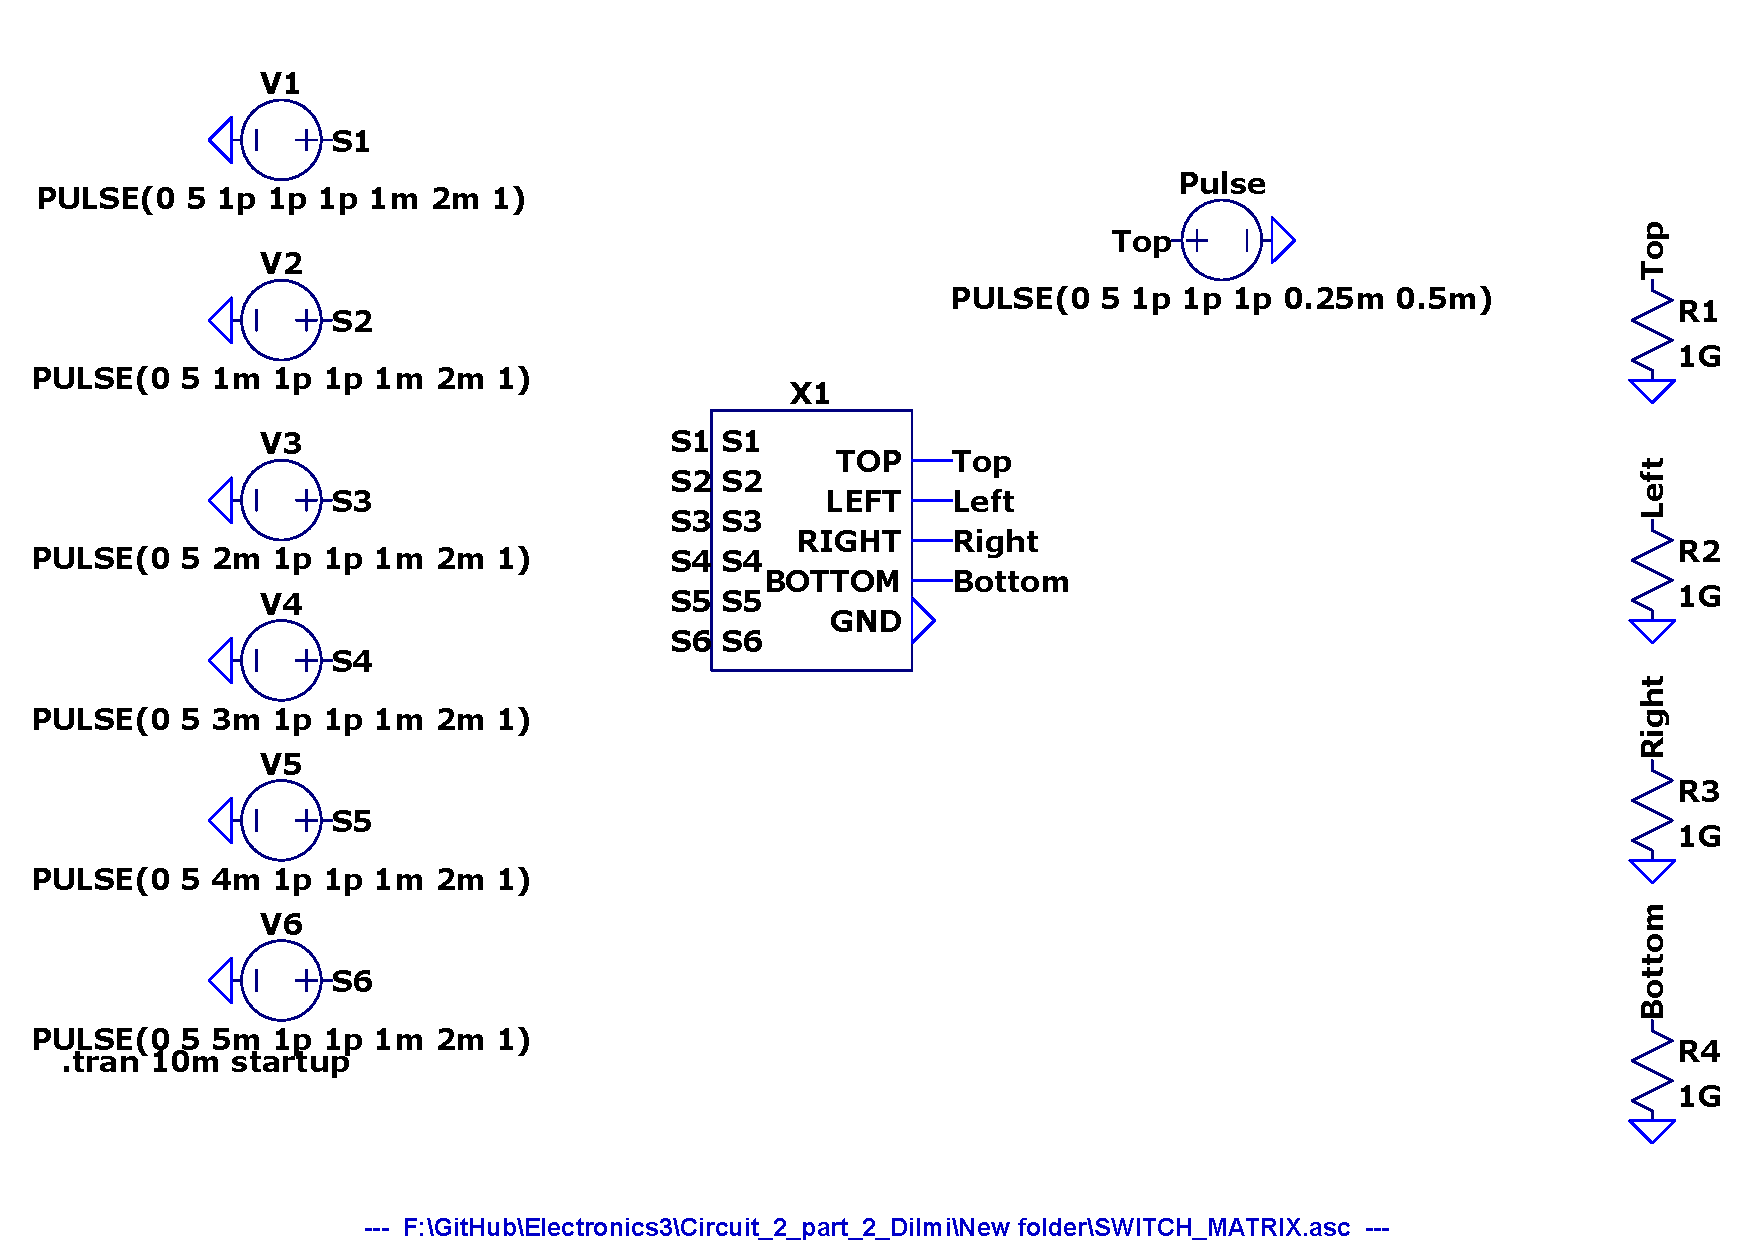
\includegraphics[scale=0.4]{figures/2part2/block.pdf}
	\caption{Designed single switch matrix block}
\end{figure}

Finally the functionality of the circuit was checked by giving pulses to left, right, top, and bottom corners separately and switching on the switches at different periods.

\begin{figure}[H]
	\centering
	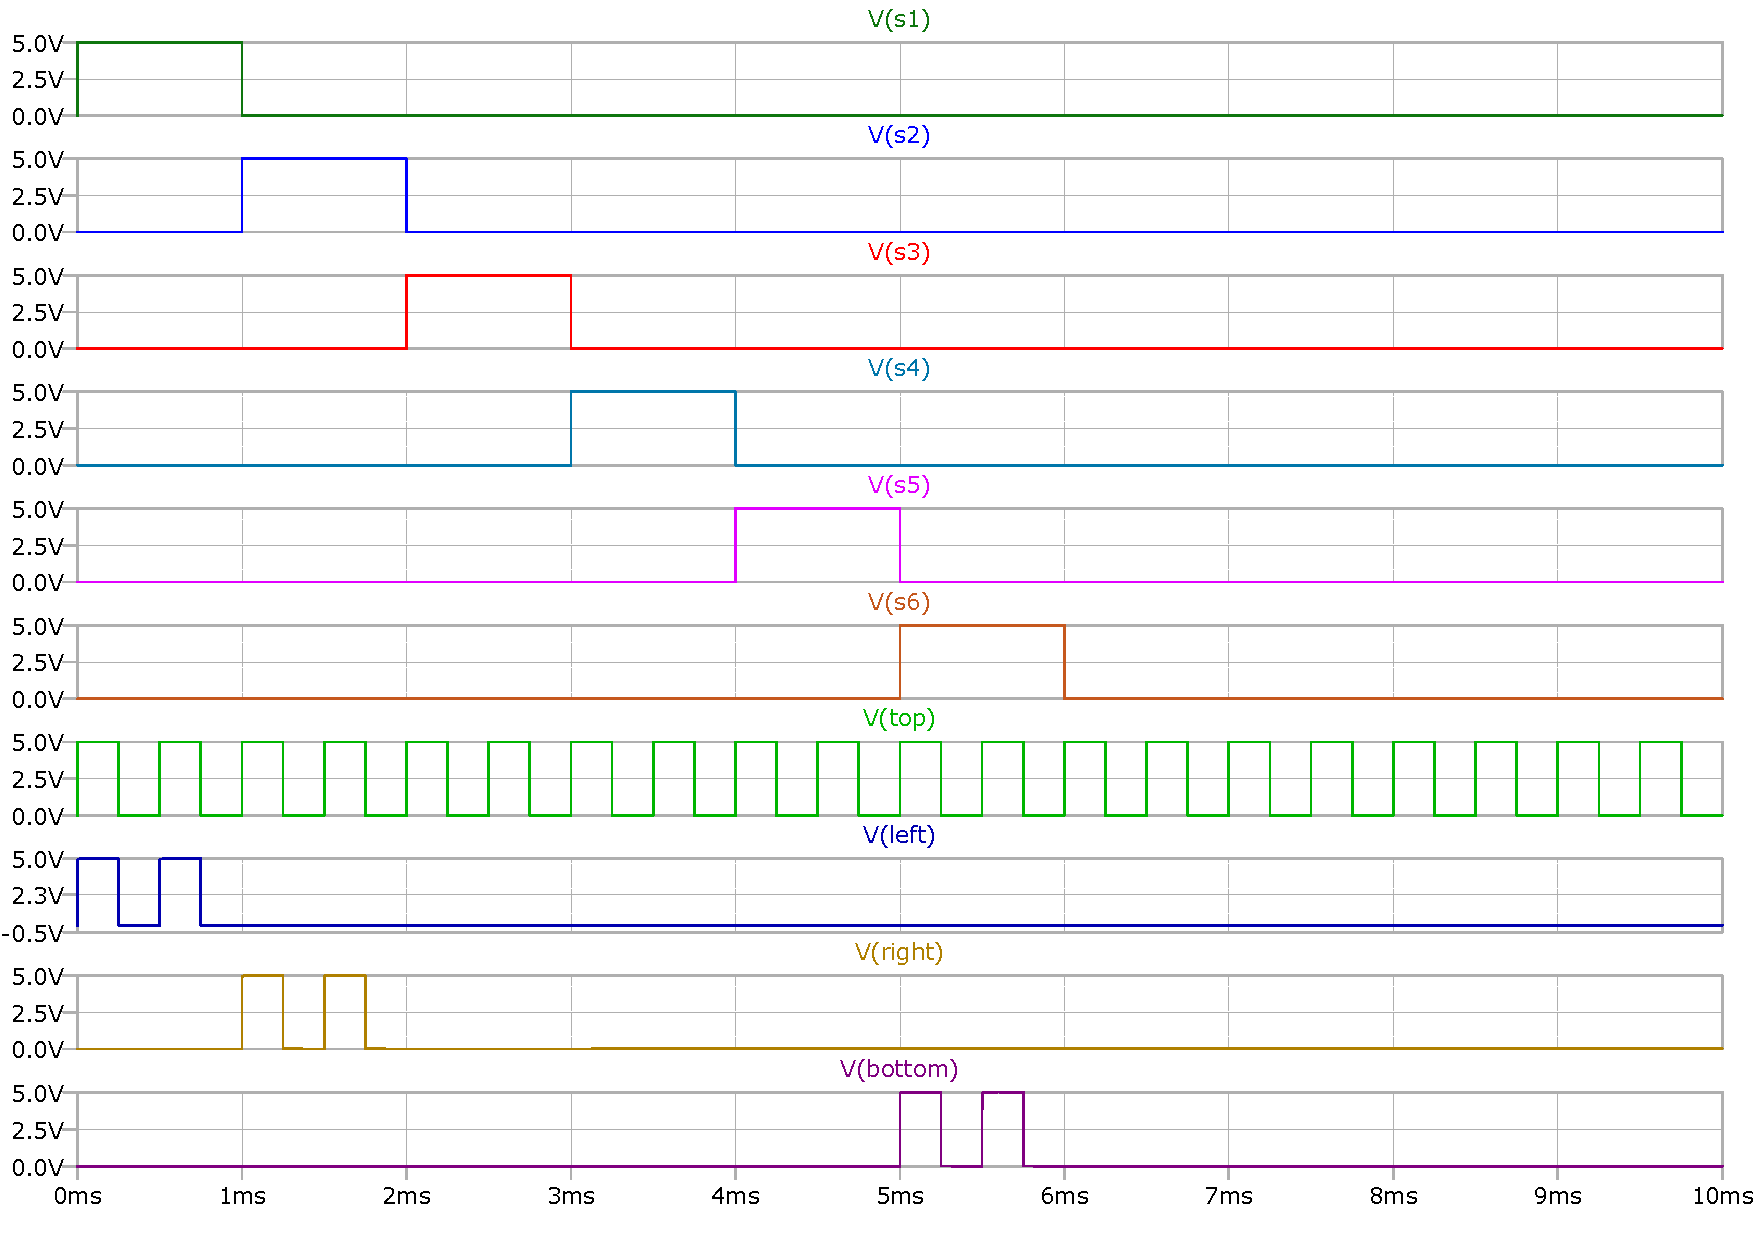
\includegraphics[scale=0.5]{figures/2part2/top.pdf}
	\caption{Waveforms when the top terminal is fed with a pulse}
\end{figure}

\begin{figure}[H]
	\centering
	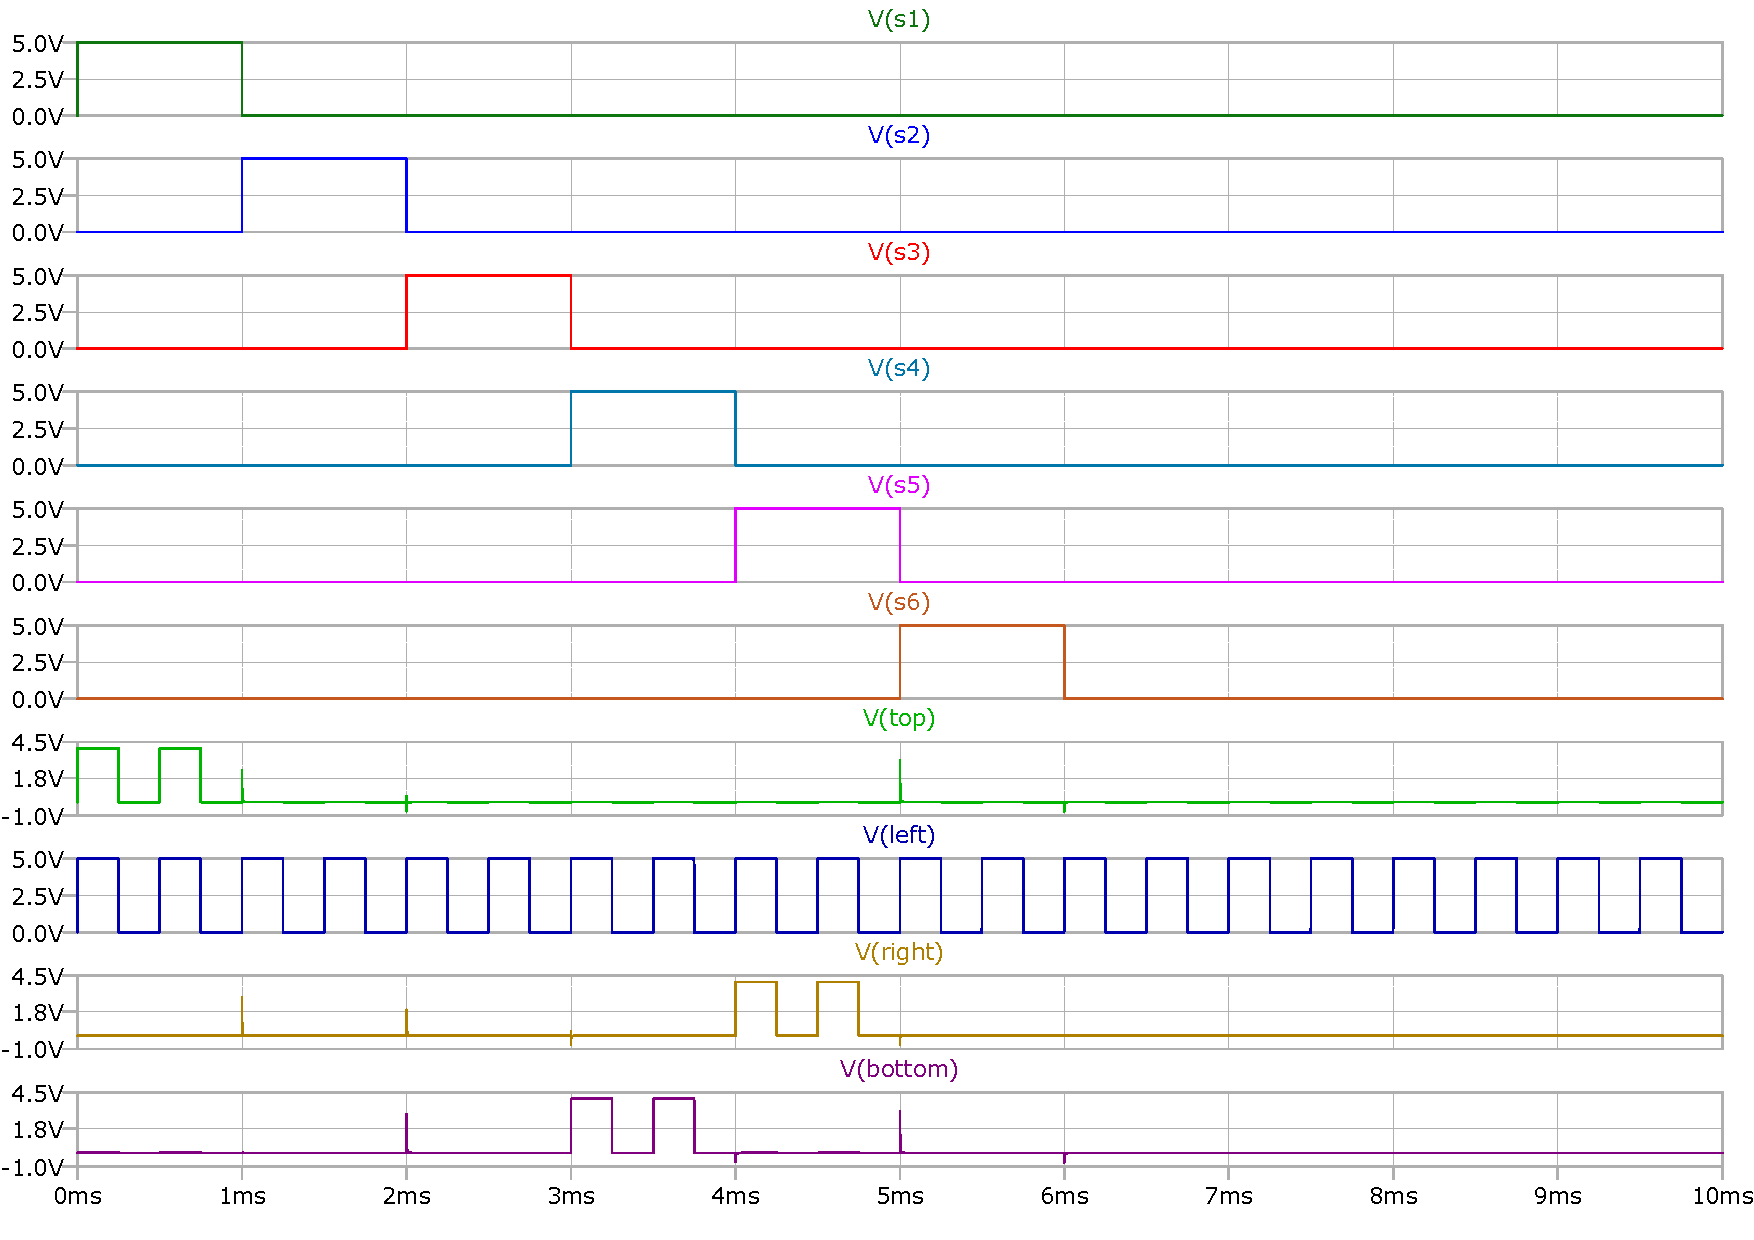
\includegraphics[scale=0.5]{figures/2part2/left.pdf}
	\caption{Waveforms when the left terminal is fed with a pulse}
\end{figure}

\begin{figure}[H]
	\centering
	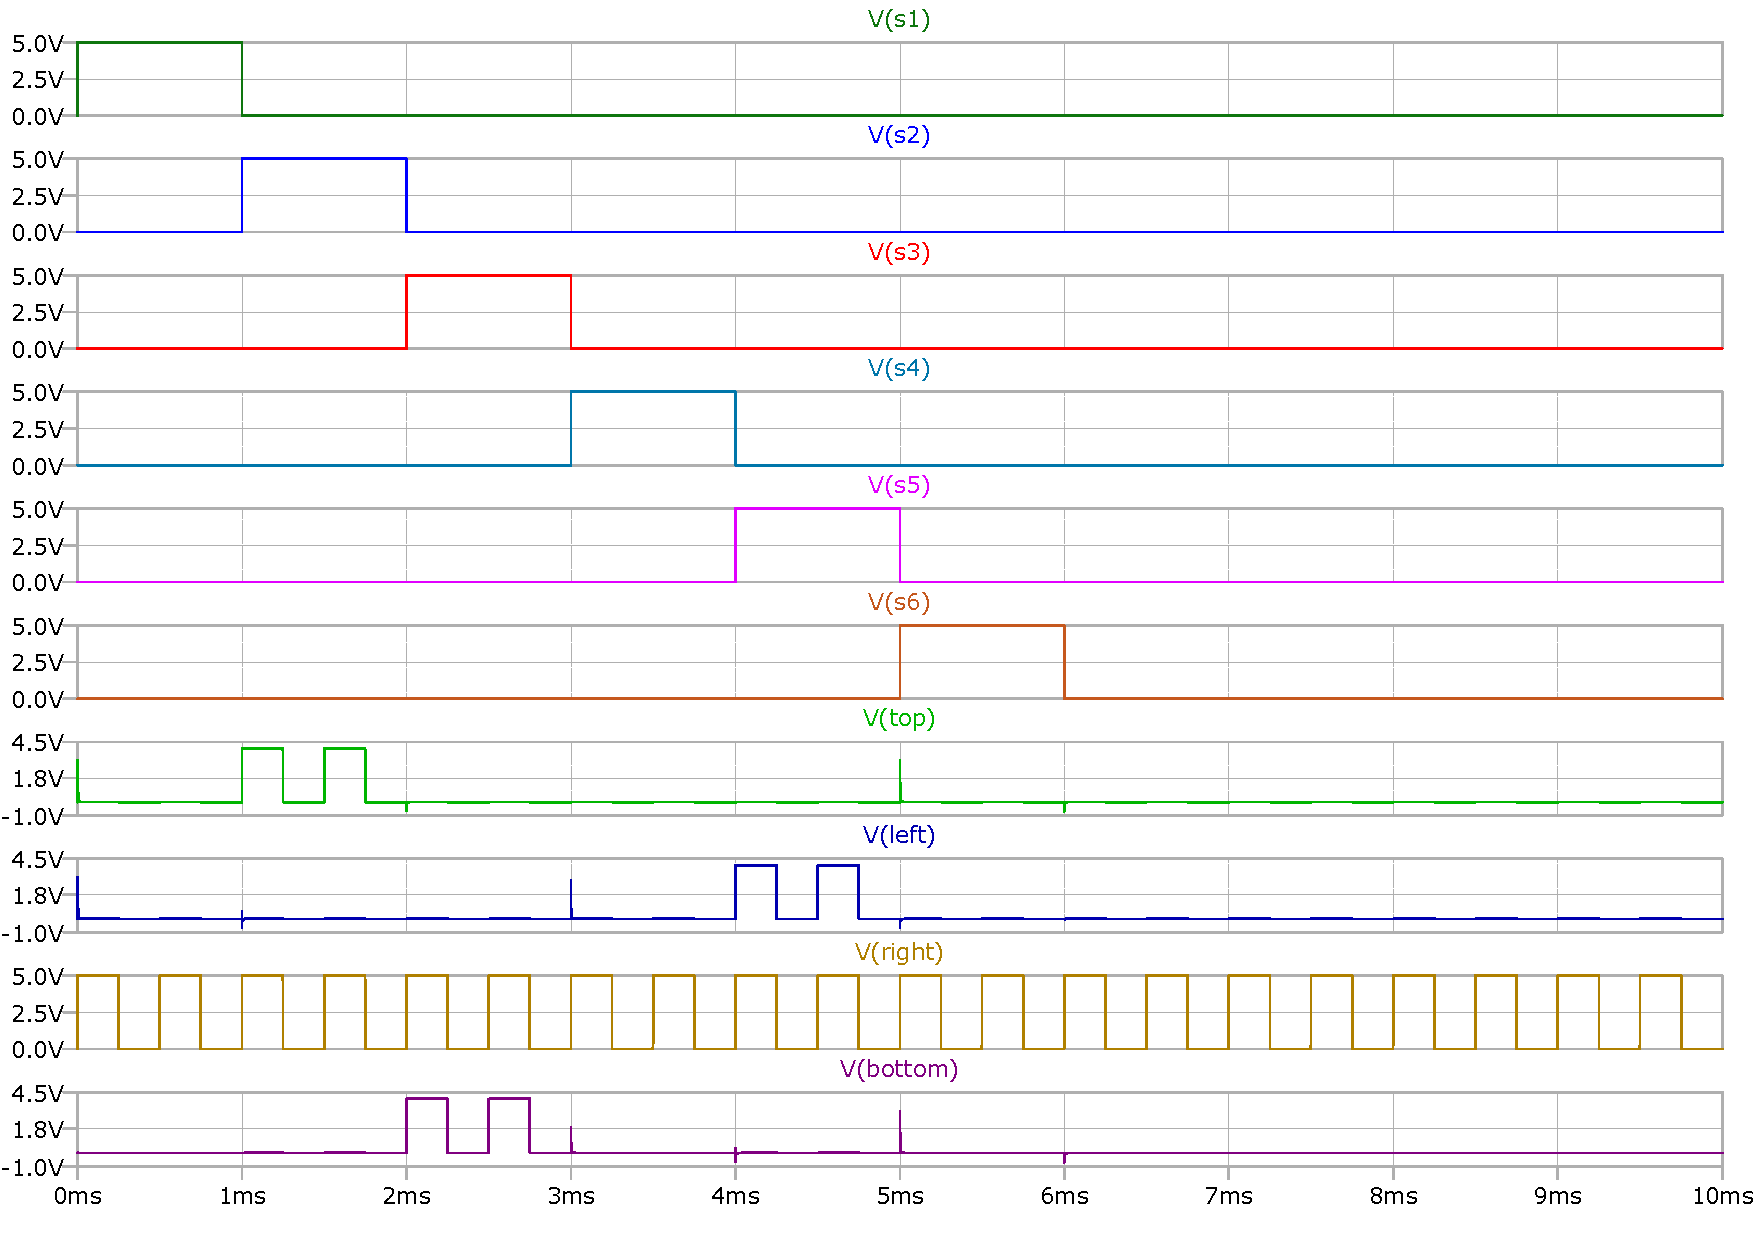
\includegraphics[scale=0.5]{figures/2part2/right.pdf}
	\caption{Waveforms when the right terminal is fed with a pulse}
\end{figure}

\begin{figure}[H]
	\centering
	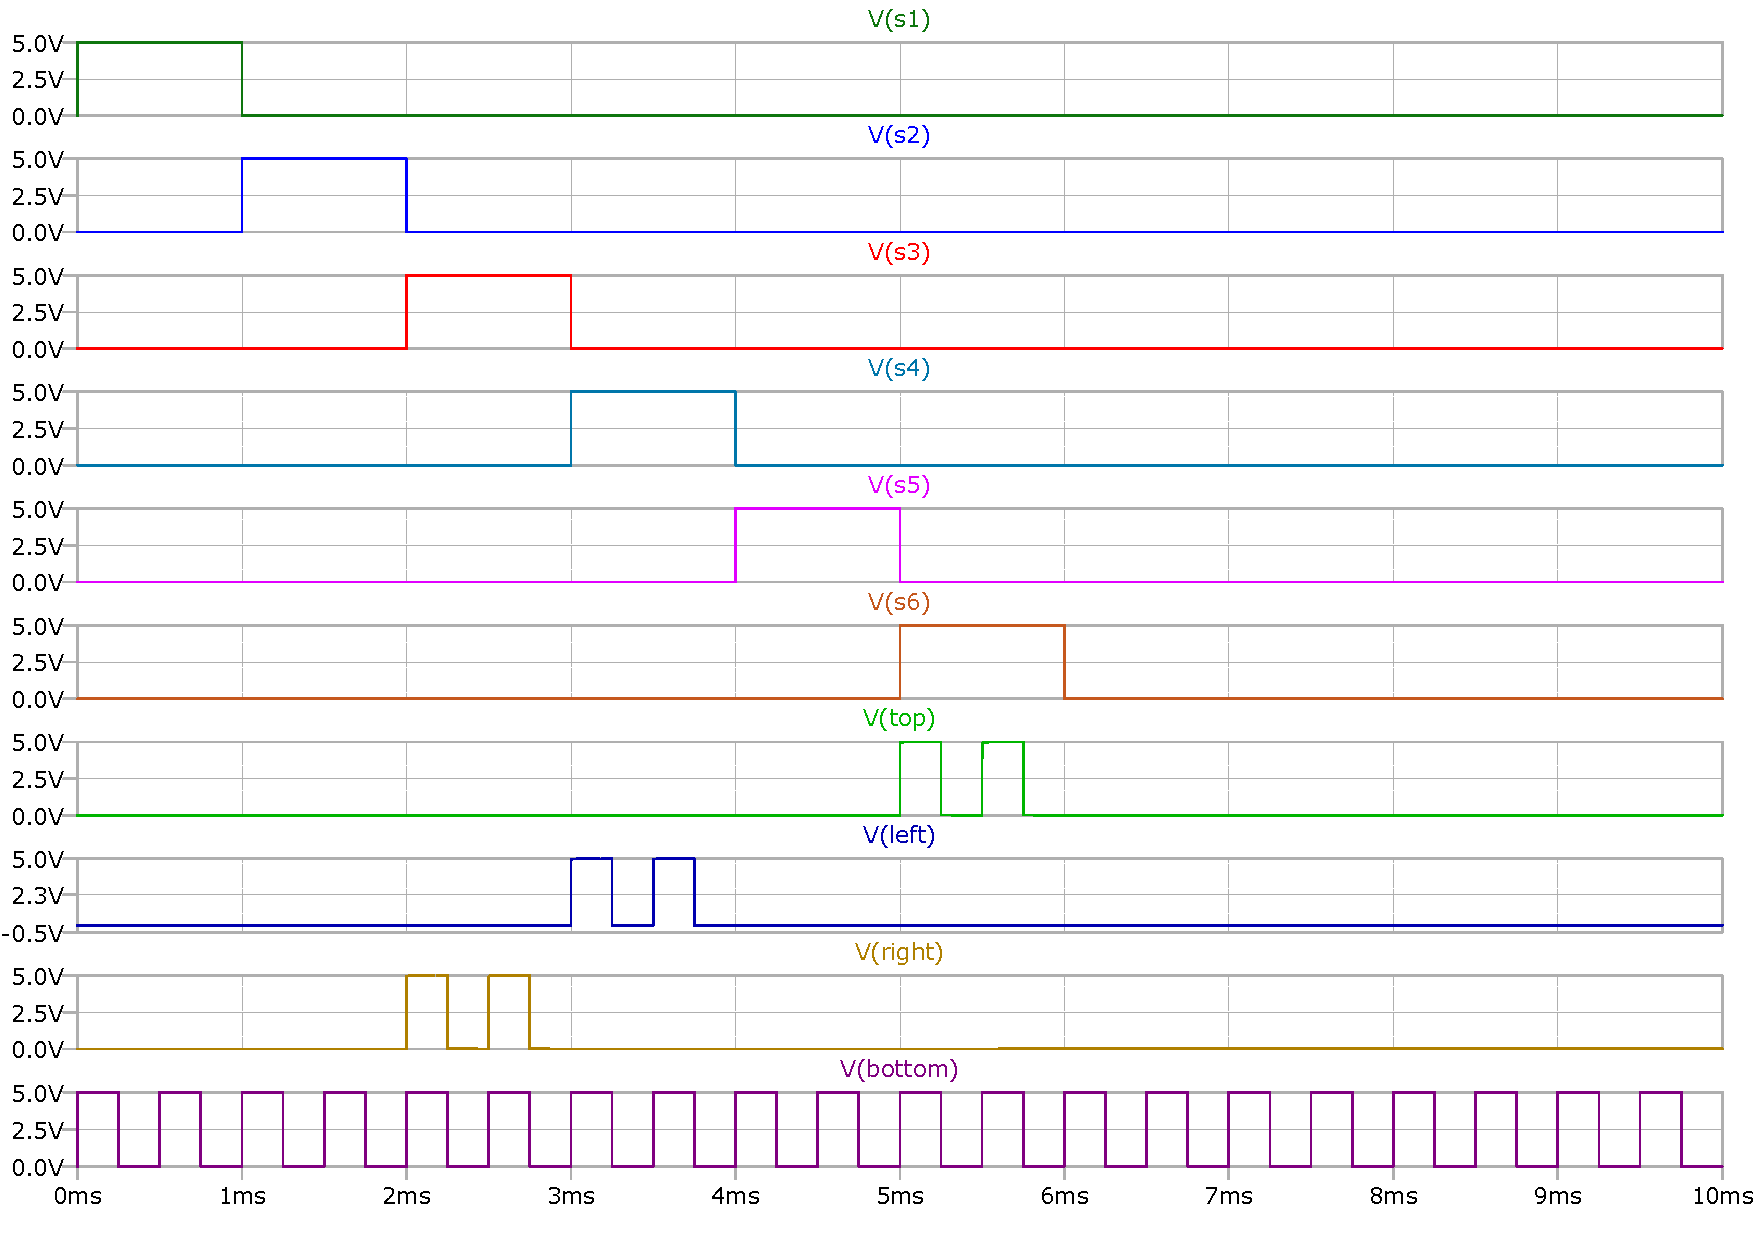
\includegraphics[scale=0.5]{figures/2part2/bottom.pdf}
	\caption{Waveforms when the bottom terminal is fed with a pulse}
\end{figure}


\hrule
\subsection{Part 3}
\textbf{Objective}: \textit{Design a PLD that can be used to design any 3 input
combinational circuit.}\\

The task was to design a PLD circuit capable of implementing any three input combinational circuit. The truth-table of any three input combinational circuits will be as below.\\

\begin{table}[H]
\centering
	\begin{tabular}{|c |c| c| c|}
		\hline
		A&B&C& Output\\\hline
	0 & 0 & 0 & $S_1 $ \\
	0 & 0 & 1 & $S_2$ \\
	0 & 1 & 0 & $S_3$ \\
	0 & 1 & 1 & $S_4$ \\
	1 & 0 & 0 & $S_5$ \\
	1 & 0 & 1 & $S_6$ \\
	1 & 1 & 0 & $S_7$ \\
	1 & 1 & 1 & $S_8$ \\\hline\hline
	\end{tabular}
\caption{The truth-table of any three input combinational circuit}
\end{table}

Outputs $S_1$, $S_2$,...., $S_8$ differ with the combinational circuit. So we can write an expression for the combinational logic circuit using the 8 minterms. Which minterms to be selected differ according to the S1, S2,...., S8. If any $S_i$ is 1 then the corresponding minterm is taken into the sum of products expression. If Si is 0 that corresponding minterm is discarded.\\

So we can build the PLD with a fixed AND plane which has all eight minterms and a programmable OR plane which can be programmed using Si terms. So our PLD becomes a PROM.\\

Before building the PLD the AND plane and OR plane should be created. For the fixed AND plane, we need eight minterms. A minterm is a product of any three of $A$, $\overline{A}$, $B$, $\overline{B}$, $C$ or $\overline{C}$. So we need three input and gate. We configured a three-input AND gate using NAND, NOR, and NOT gates as below for better efficiency.\\

\[ A.B.C = \overline{\overline{A.B.C}} = \overline{\overline{A.B} + \overline{C}} \]

Using this expression we constructed the 3 input AND gates using a minimum number of logic gates.\\

\begin{figure}[H]
	\centering
	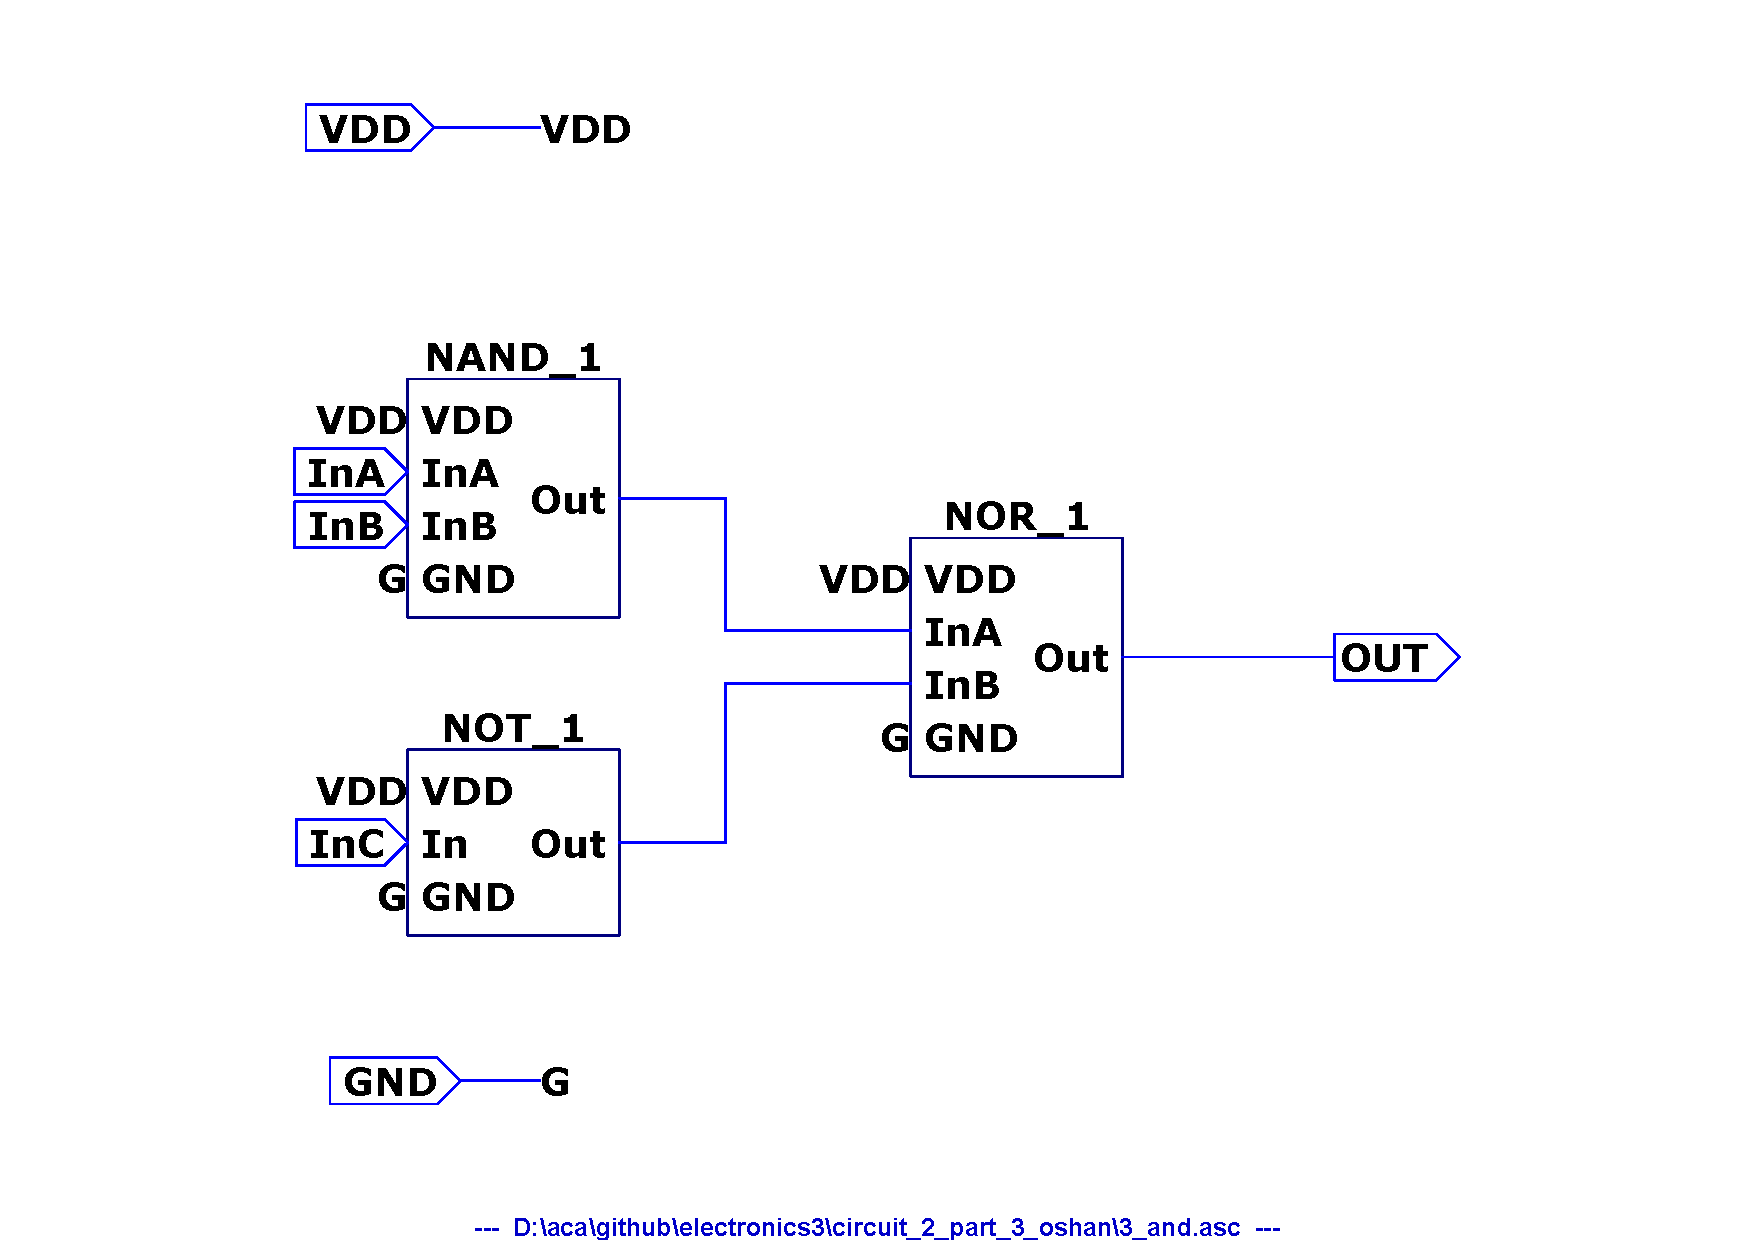
\includegraphics[scale=0.5]{figures/Figure332.pdf}
	\caption{Implementing the three-input AND gate using NOR, AND, and NOT gates.}
\end{figure}

Using seven separate OR gates( 7 NOR gates + 7 NOT gates) to implement the OR plane, increases complexity and the latency of the circuit by a huge factor. Instead, we can simplify the expression and use a minimum number of gates as below.\\

\[
\begin{split}
 & = S_1 + S_2 + S_3 + S_4 + S_5 + S_6 + S_7 + S_8\\
 & = \overline{\overline{S_1 + S_2 + S_3 + S_4 + S_5 + S_6 + S_7 + S_8}}\\
 & = \overline{\overline{\left( S_1 + S_2 + S_3 + S_4 \right)}. \overline{\left( S_5 + S_6 + S_7 + S_8 \right)}}\\
  & = \overline{\overline{\left( S_1 + S_2\right)} .\overline{\left( S_3 + S_4 \right)}. \overline{\left( S_5 + S_6\right)}.  \overline{\left( S_7 + S_8 \right)}}\\
    & = \overline{\overline{\left( S_1 + S_2\right)} .\overline{\left( S_3 + S_4 \right)}}+ \overline{\overline{\left( S_5 + S_6\right)}.  \overline{\left( S_7 + S_8 \right)}}\\
    & = \overline{\overline{ \overline{\overline{\left( S_1 + S_2\right)} .\overline{\left( S_3 + S_4 \right)}}+ \overline{\overline{\left( S_5 + S_6\right)}.  \overline{\left( S_7 + S_8 \right)}} }}
\end{split}
\]

Using this expression we were able to build an OR plane with a minimum number of components as below.\\

\begin{figure}[H]
	\centering
	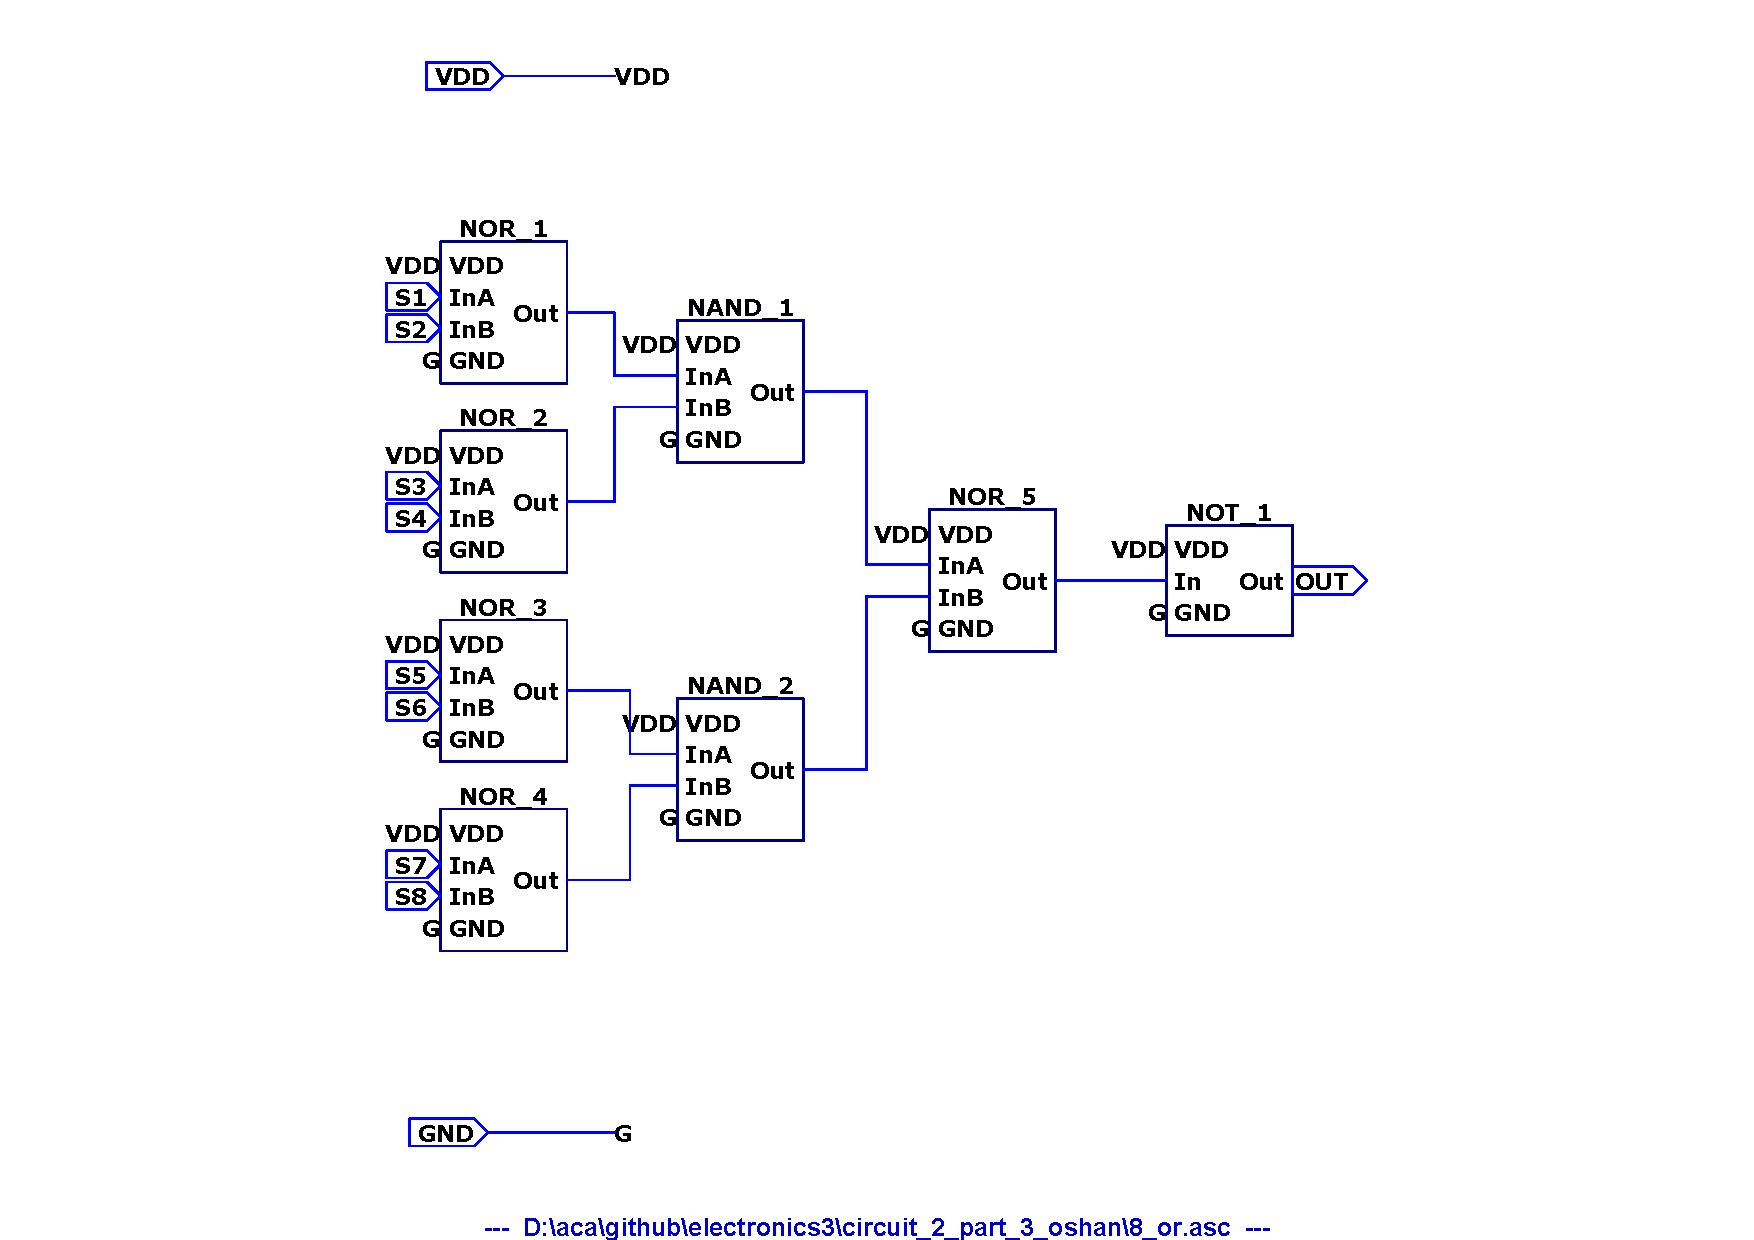
\includegraphics[scale=0.5]{figures/Figure333.pdf}
	\caption{Implementing the OR plane}
\end{figure}


Instead of using a total of 14 logic gates, now we have implemented it using only 8 logic gates. This reduces the latency and complexity by a huge factor.\\

PROM is constructed as below\\

\begin{figure}[H]
	\centering
	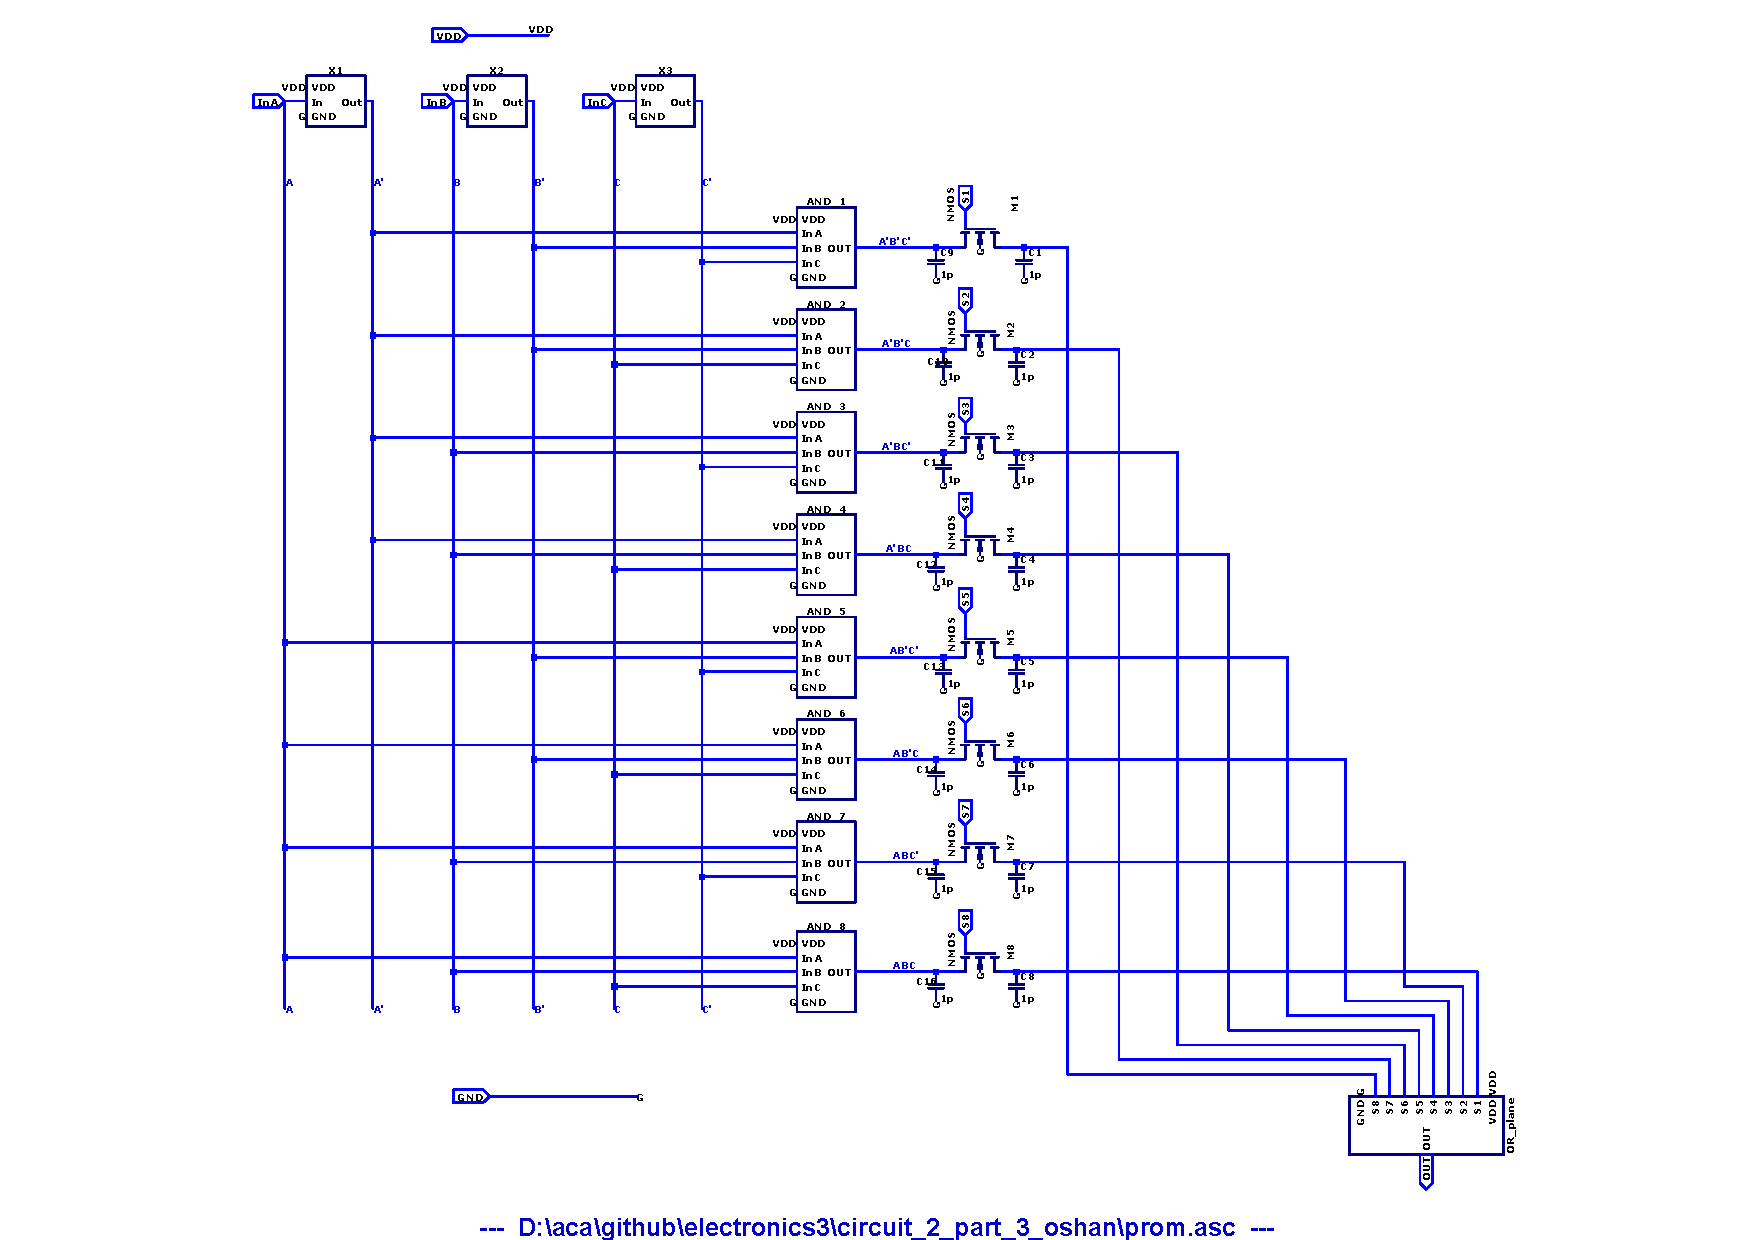
\includegraphics[scale=0.5]{figures/Figure334.pdf}
	\caption{PROM circuit}
\end{figure}


We have used nmos transistors as switches which choose, which minterms are taken into the sum of products. We didn’t choose passgates as switches as it increases the complexity and the latency of the circuit.\\ 

We tested the circuit for different combinational circuits by configuring Si switches. Below we have configured the PROM as a simple NOR gate.\\


\begin{figure}[H]
	\centering
	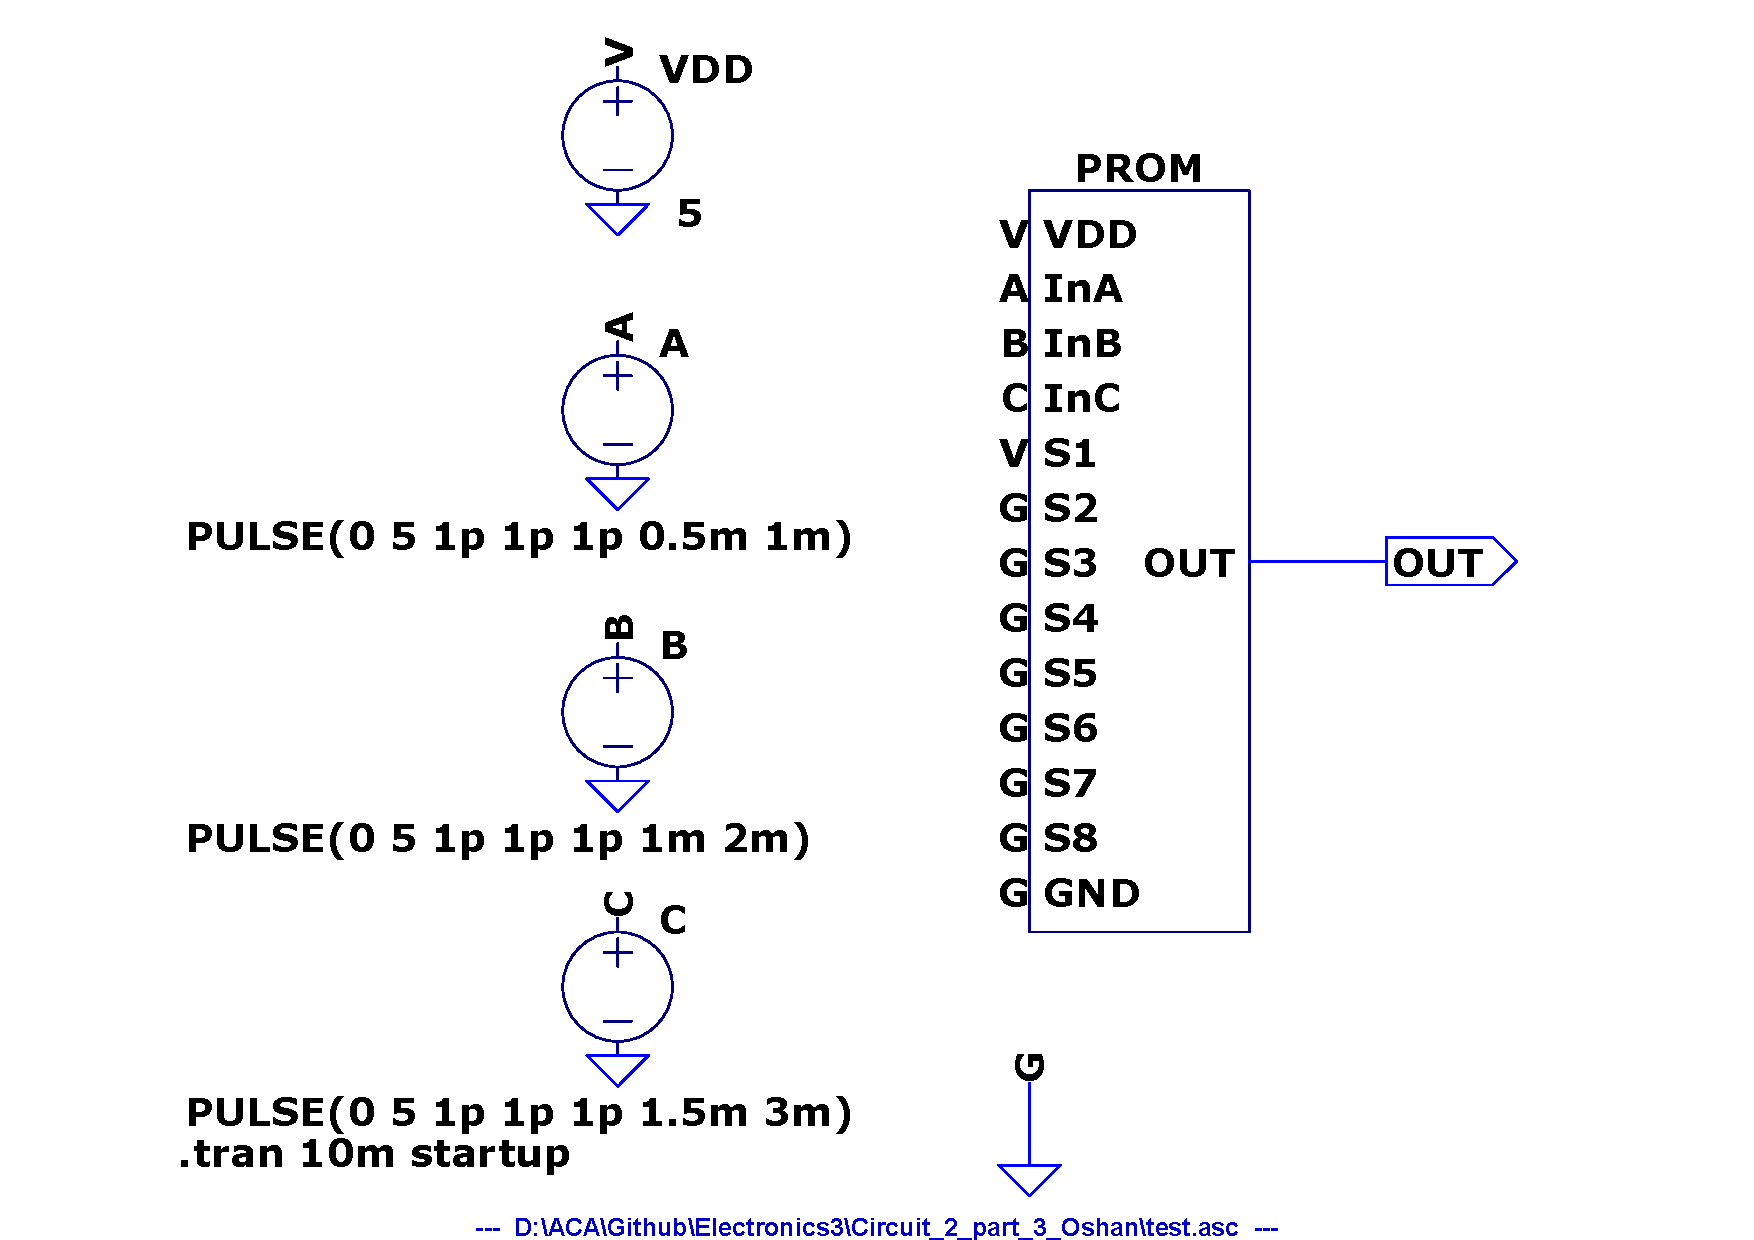
\includegraphics[scale=0.5]{figures/Figure335.pdf}
	\caption{PROM configured as a NOR gate}
\end{figure}

Results were as below,
\begin{figure}[H]
	\centering
	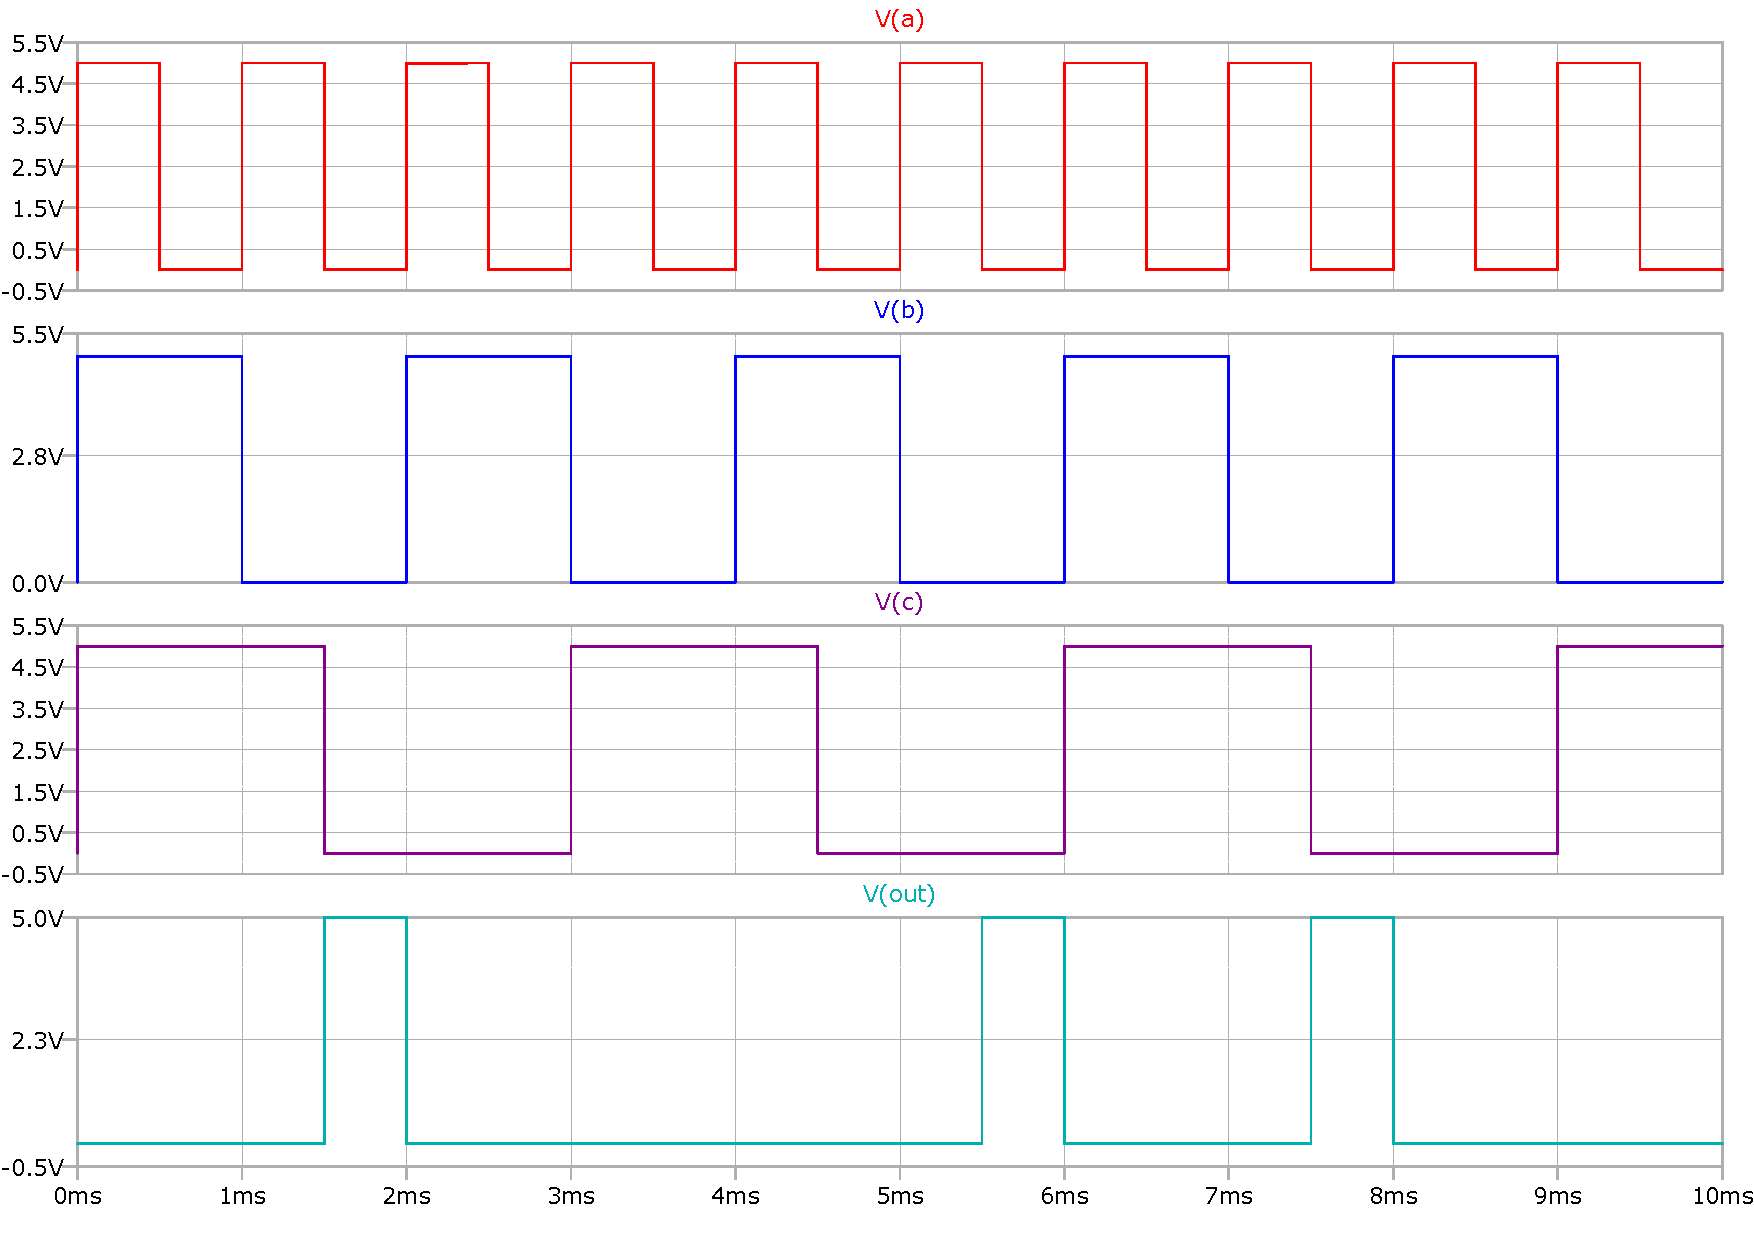
\includegraphics[scale=0.5]{figures/Figure336.pdf}
	\caption{Results of PROM configured as a NOR gate}
\end{figure}

We can observe that the PROM is functioning correctly.

\vfill
\hrule
{\scriptsize
\bibliographystyle{plain}
\bibliography{refer}
}
%---------------------------------------------------------------------------
\end{document}
